\documentclass[12pt]{article}
\usepackage{graphicx} % for inserting images
\usepackage[utf8]{inputenc} % for good practice
\usepackage{amsmath} % for equations
\usepackage{amsfonts}
\usepackage{hyperref}
\usepackage[ruled,linesnumbered]{algorithm2e}
\usepackage{setspace}
\usepackage{siunitx}
\usepackage{csquotes}
\usepackage{changepage}
\usepackage{subfig}
\usepackage{url}
\usepackage{subcaption}
\usepackage{rotating}
\usepackage{tikz}
\sisetup{output-exponent-marker=\ensuremath{\mathrm{e}}}
\usepackage[
backend=biber,
sorting=ynt
]{biblatex}
\addbibresource{references.bib}

\title{\textit{Document Classification in \\Public Administration}}
\author{Gugole Nicola\\Pasquali Alex\\Piccoli Elia}
\date{September, 2021}

\begin{document}
\begin{titlepage}
	\maketitle
	\pagenumbering{gobble}
   \begin{center}
	\vspace{0.5cm}
       Final project for the\\ \textit{Human Language Technologies}\\ course
       \vfill	     
       
\includegraphics[width=0.2\textwidth]{unipi.png}\\
       University of Pisa\\
       Artificial Intelligence\\
       A.Y. 2020/2021\\
   \end{center}
\end{titlepage}
\newpage
{\small\tableofcontents}
\pagenumbering{arabic}
\newpage

\section{Project Purpose}\label{sec:projectpurpose}
The project was developed in association with \textit{Compagnia Trasporti Toscana (CTT)}, which is the company that handles the public transportation in Tuscany, and Doc. Riccardo Franchi (Corporate Manager), who was our reference inside the company.
The focus of the project was to improve the document archiving process in compliance with the \textit{Protocollo Informatico Italian} law. In fact, the user of public administration, in order to archive a protocol, has to fill various fields (\hyperref[fig:interface]{\textbf{Figure 3}}), in particular: needs to write a summary of the contents of the document (\textit{Oggetto}), pick the correct document repository for the office (\textit{Contenitore}) and then choose the correct class among many. The different classes are stored in a hierarchical structure (\textit{Titolario}, \hyperref[fig:classinterface]{\textbf{Figure 4}}), where going from higher to lower levels a more precise description of the class is provided. The user, in order to select the class, has to navigate through the various levels of the hierarchy. Each office is responsible for the administrative processes identified by the classes of its competence. This results in a mechanic and repetitive task, that the user must do each time a new protocol arrives. Obviously, this process is not error-free since it is heavily influenced by the user competence, each error affect the quality of the administrative process.\\

The purpose of the project is to speedup and provide soundness to the class selection task providing the user with a suggestion formed of a small set of classes where the document is more likely to be classified.
In this way, without going through the hierarchy, the user is able to exploit the model prediction.
In order to properly build the model architecture a key point was to define input and output. The \textit{output} can be easily defined as a distribution probability over the different classes. The \textit{input}, instead, was limited to only a small subset of available information. As a matter of facts, the input is composed by two elements: \textit{Oggetto} and \textit{Contenitore}.
\hyperref[sec:model-desc]{\textbf{Section \ref{sec:model-desc}}} will provide more information on how the two different fields are handled. An important aspect that will play a key role is the \textit{inference time}, in fact the model needs to be fast in order to give an almost instant feedback to the user that would otherwise need to search among the hierarchy.\\

The analysis will be divided into different sections. Starting from an in depth analysis of the dataset in \hyperref[sec:dataset]{\textbf{Section \ref{sec:dataset}}}, followed by the analysis of the two main task of the project. \hyperref[sec:1lev-model]{\textbf{Section \ref{sec:1lev-model}}} will cover the easier task using only the first level of the classes hierarchy resulting in a probability distribution of \textit{15} elements. \hyperref[sec:2lev-model]{\textbf{Section \ref{sec:2lev-model}}}, instead, will focus on the second level of the tree leading to \textit{118} possible classes. The remaining sections will analyze different architectures, the results over a new set of data and some final considerations.

\section{Dataset Preprocessing}\label{sec:dataset}
\textit{CTT} company kindly offered us its entire dataset, with the hard constraint of taking the data starting from January 2018 because of a change of class tree which happened at the time. The raw dataset consisted of \textbf{~100000} samples and needed a meticolous preprocessing to avoid privacy issues. Further parsing was also needed to generalize otherwise futile vocabulary entries.

\subsection{Dataset Features Extraction}
The dataset was composed initially of many features comprising date of insertion, object, office, class code, class name and various ids as external keys to other dataset tables.\\Of these only a subset was kept for the model input, as explained in \hyperref[sec:projectpurpose]{\textbf{Section \ref{sec:projectpurpose}}}. The dataset is therefore composed of 4 features:
\begin{itemize}
    \item \textbf{Oggetto:} string defining a summary of the document which is being classified.
    \item \textbf{Contenitore:} string representing the document repository where the protocol is archived. From now on, for simplicity sake, the document repository will be referred to as \textit{office}.
    \item \textbf{PrimoLivello:} integer ranging from 1-15, ground truth for first level classification.
    \item \textbf{SecondoLivello:} integer with a value range depending on the first level (each first level may have a different subtree), combined with \textit{PrimoLivello} gives a ground truth for second level classification.
\end{itemize}

\subsection{Dataset Cleaning}
A series of operations was applied in order to privatize and generalize the data as much as possible, trying at the same time to keep highest possible variability for better learning.

Exploring the samples and discussing with Doc. Franchi lead to the individuation of personal data as well as offices for which the task is useless. Two situations in particular lead to a first skimming of the dataset:
\begin{itemize}
    \item A specific class (\textit{Permessi sindacali}) contained a notable amount of full names, and was therefore dropped under Doc. Franchi advice. 
    \item An ensemble of protocols all involving \textit{Fatture} was dropped due to the uselessness of a classifier in that case. The documents involving these protocols are in fact not inserted by hand but by an automatized process.
\end{itemize}
This first process left us with a dataset composed of \textbf{60509} samples, which we furthered cleaned and treated by transforming the input features (\textit{Oggetto} and \textit{Contenitore}) into lower case strings and by stripping the resulting samples from any unnecessary leading/trailing whitespace. 

\subsection{Dataset Balancing} \label{sec:dataset-balancing}
The implicit different load of documents per class in a real world application such as this one leads to a not surprising fact, the unbalancing in number of samples per class. An unbalanced dataset is not ideal for the task, since the model will have a disproportion of learning material with a consequent lower precision in less populated classes. \\We therefore opted for a balancing process on the dataset, applying a careful stratification to low populated classes and a reduction to exaggeratedly populated ones. The main aim of the process was to result in a more balanced first level dataset (the second level of the tree is too unbalanced and sparse) while maintaining the data distribution. 
\begin{itemize}
    \item \textbf{Stratification:} applied to class 3,5,11 and 12. Unfortunately we could not automatically generate new samples in the \textit{Oggetto} field because of its textual nature, nevertheless we tried to higher the number of samples and their variability by creating new rows where \textit{Oggetto} and \textit{Contenitore} are chosen independently and randomly from the pool of \textit{Oggetti} and \textit{Contenitori} of a specific second level class. This augmentation assured the correctness of the dataset both for the first level and the second level task. 
    \item \textbf{Reduction:} applied to class 6,14. Randomly chosen samples were dropped. Randomization was preferred to cutting beginning/end of dataset for a higher probability in maintaining the interclass distribution.
\end{itemize}
The result of the balancing process can be appreciated in \hyperref[fig:before]{\textbf{Figure 1a}} and \hyperref[fig:after]{\textbf{Figure 1b}}.
\begin{figure}[!tbp]
  \centering
  \subfloat[Before balancing]{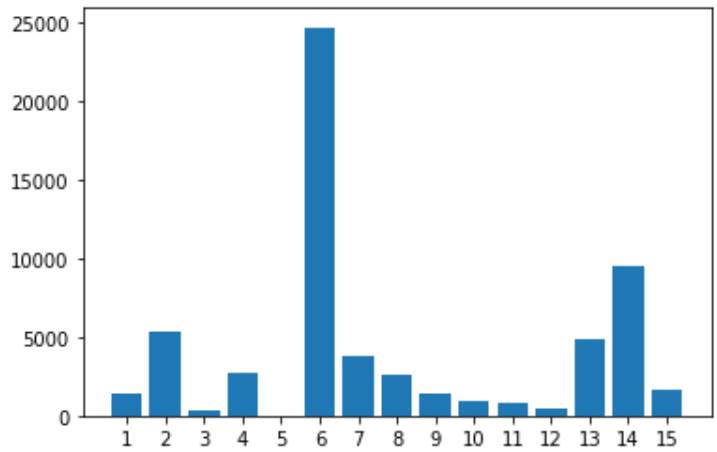
\includegraphics[width=0.4\textwidth]{before_balancing.png}\label{fig:before}}
  \hfill
  \subfloat[After balancing]{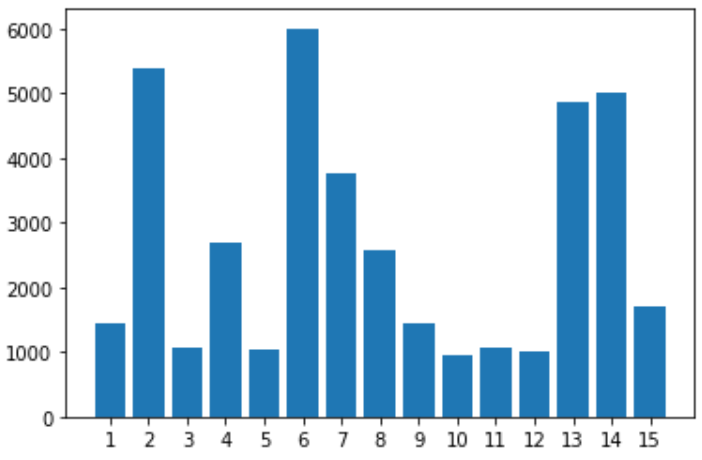
\includegraphics[width=0.4\textwidth]{after_balancing.png}\label{fig:after}}
\caption{Class distribution}
\end{figure}

\subsection{Dataset Parsing}
Data parsing is a fundamental aspect when working with Natural Language, therefore we applied a last series of filtering and mapping to our data before feeding it to the model. Because of the predetermined and fixed range of values for \textit{Contenitore}, we decided to apply the parsing only to the \textit{Oggetto} field, definitely more dynamic than the other. The treating of \textit{Contenitore} will be further discussed in \hyperref[sec:office-module]{\textbf{Section 3.1.2}}.
\\The dataset has therefore to pass through a last procedure before being ready for training:
\begin{itemize}
    \item \textbf{Filtering:} Generalizing the data from futile or private information, replacing all dates, hours, emails and generic numbers with more general tokens, namely \textless DATE\textgreater, \textless HOUR\textgreater, \textless EMAIL\textgreater, \textless NUMBER\textgreater. Particular care was put into the email processing, a process which was manually checked to ensure the avoidance of personal data in the final training dataset, which might have happened due to the possible incorrectness of human written text.
    \item \textbf{Tokenization:} Splitting the data in single words and removing punctuation. A particularity here stands in the need for a fixed number of words in the processed \textit{Oggetto} field. The use of a Transformer (further introduced in \hyperref[sec:object-module]{\textbf{Section 3.1.1}}) implies in our case an Embedding Layer for which a fixed input dimension is required. We therefore studied and analyzed the \textit{Oggetto} length variability and opted for a sequence length of \textbf{30 words}. The decision came from a statistical analysis (a summary can be appreciated in \hyperref[fig:objectlength]{\textbf{Figure 2}}) merged with the will of being as indulgent as we can and maintain as much information as possible in the sentence. Consequently, sentences with more than 30 words are truncated and in the opposite case are filled to reach the correct length with special padding tokens (\textless PAD\textgreater).
    \item \textbf{Encoding:} After collecting all dataset tokens a vocabulary is created and so is a mapping between token and integer. This allows for a fast encoding procedure, transforming the input sentence in an integer array which can be directly fed to the model (if a word is not present in the vocabulary it is replaced with a special token, \textless UNK\textgreater).
\end{itemize}
\begin{figure}[ht!]
    	    \begin{center}
        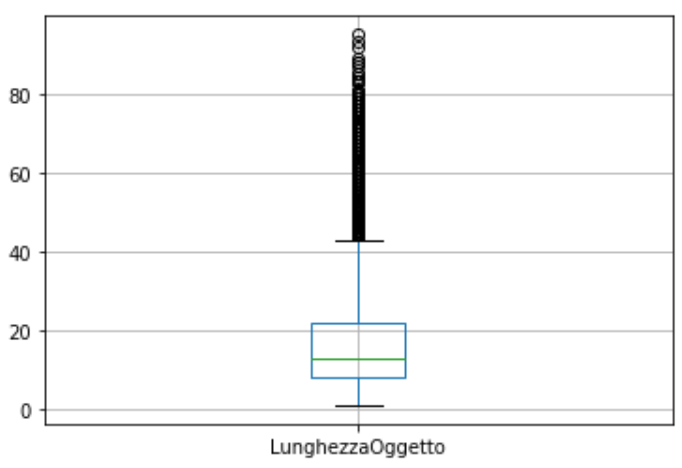
\includegraphics[width=0.7\textwidth]{object_length.png}
            \end{center}
        \label{fig:objectlength}
        \caption{Object length boxplot}
\end{figure}

\section{First Level Model}\label{sec:1lev-model}
In this section is described the model used to perform the classification in the first (highest, most general) level of the hierarchy of classes.

\subsection{Model Description}\label{sec:model-desc}
The class of each protocol depends on two aspects:
\begin{itemize}
    \item \textbf{Oggetto}: subject of the document, inserted by the human operator at classification time.
    \item \textbf{Contenitore}: archiving office for the protocol. Each office may archive different categories of documents, which, therefore, belong to different classes.
\end{itemize}
These two attributes are treated differently, by two different sub-models (\textbf{object module} \ref{sec:object-module} and \textbf{office module} \ref{sec:office-module}) whose outputs will be combined and fed to a multi-layer perceptron (MLP) that will perform the final classification.

\subsubsection{Object module}\label{sec:object-module}
Due to the textual nature of \textit{Oggetto} attribute, that can be seen as a summary of the content of the document, it is important to capture its semantics in order to understand the general matter of the document itself and perform a meaningful classification.\\
For this reason, the choice was to start from a standard \textbf{Transformer} \cite{attention_is_all_you_need, pytorch_transformer}, that is formed by a stack of encoders and decoders that work as follows:
\begin{itemize}
    \item \textbf{Encoders:} each one of the encoders of the stack has two sub-layers: the first is a \textit{multi-head self-attention} mechanism, and the second is a simple, position-wise fully connected feed-forward network.
    \item \textbf{Decoders:} each decoder in the stack, in addition to the two sub-layers in each encoder layer, the decoder inserts a third sub-layer, which performs multi-head attention over the output of the encoder stack.
    \item \textbf{Multi-head self-attention:} Instead of performing a single attention function, \textit{queries}, \textit{keys} and \textit{values} are linearly projected $h$ times with different, learnt, linear projections. The attention function is performed in parallel for each of these queries, keys and values.
\end{itemize}
Now, since the task is a classification (and not, for example, a sequence-to-sequence transduction), only the encoders of the transformer are needed.\\
The model used in the task, so, is formed by an embedding layer \cite{pytorch_embedding} followed by a \textit{TransformerEncoder} \cite{pytorch_transformerencoder}, that is a stack of encoders as described in \cite{attention_is_all_you_need}.

\subsubsection{Office module}\label{sec:office-module}
The information about the office that performs the classification is categorical, so, from textual data, it gets 1-hot encoded.
This, anyway, is not beneficial for the model, because the information would be very sparse, for this reasons \textbf{office module} serves as an embedder used to move towards a dense representation.
\paragraph{Architecture}
This embedder is built as a MLP with 3 layers, all with a ReLU activation function. In particular:
% an input layer of 20 units (i.e. the dimensionality of the 1-hot encoding), a hidden layer of 10 units to form an "information bottleneck" and an output layer of 128 units (i.e. the chosen dimensionality of the encoding).
\begin{itemize}
    \item input layer: 20 units, i.e. the dimensionality of the 1-hot encoding of the office.
    \item hidden layer: 10 units, it reduces the dimensionality to serve as an "information bottleneck".
    \item output layer: 128 units, i.e. the chosen dimensionality of the embedding.
\end{itemize}
\paragraph{Training of the embedder}
This embedder is trained in an \textit{encoder-decoder fashion}:
at training time, another fully-connected layer is added at the end of the embedder, whose input dimension corresponds to the embedding one (128) and its output dimension is equal to the dimensionality of the original 1-hot encoding of the office (20).
This final layer has a \textit{tanh} activation function and its purpose is to reconstruct the original 1-hot encoding.
To draw a parallel with an encoder-decoder architecture, the embedder acts as the encoder while the final layer serves as decoder.\\
During the training process, the data is passed through the full architecture (embedder + final layer) and the loss function (cross entropy) forces the model's output to be as similar as possible to the model's input.\\\\
\textbf{Notes:}
\begin{itemize}
    \item PyTorch's implementation of the cross entropy loss \cite{pytorch_crossentropy} does not necessarily want an input that is scaled in the interval $[0,1]$, as this operation is performed by the loss itself.
    \item The \textit{sigmoid} activation function in the final layer would also be good for reconstructing a 1-hot encoding, but the results were worse, therefore the final choice was the \textit{tanh}. As stated in the previous point, it is not necessary that the model's output is scaled in $[0,1]$.
\end{itemize}

\subsection{Performances}\label{sec:1-lvl-perf}
Experiments were carried out on a \textit{Lenovo Legion Y740-17IRHg} using its GPU (\textit{NVIDIA GeForce RTX 2080 Max-Q}) to speedup the training process. Pay attention that although trainings are executed on GPU, all timings reported for inference are referring to CPU execution of a trained model. 

Model training and validation have been carried out using a dataset with data coming from 2018 up to mid May 2021 using a \textit{Hold Out} validation strategy with an 80-20 split. \textit{Top 1} and \textit{Top 3} accuracy are used for model selection and \textit{Cross Entropy Loss} is used for learning because of the multi-class task. \textit{ReLU} is used throughout all the model as activation function.

An initial screening phase brought out the necessity of having a bigger chunk of the final classifier input composed of the object module (\hyperref[sec:object-module]{\textbf{Section \ref{sec:object-module}}}) with respect to the office module (\hyperref[sec:office-module]{\textbf{Section \ref{sec:office-module}}}) embedding size. The screening phase also helped with fixing other parameters, such as the \textit{Learning Rate} (after the initial trials we opted for a default \textit{Adam} optimizer), the use of a \textit{Multi-Head Attention} with 8 heads and a Transformer Encoder stack of 2 levels.

Our trials have therefore focused on attempting the varying of \textit{object embedding size}, \textit{office embedding size}, \textit{number and extension of layers in final classifier} and \textit{amount of regularization}. Most relevant results are shown in \hyperref[tb:firstlevel-hyper]{\textbf{Table \ref{tb:firstlevel-hyper}}}. All attempts\footnote{obj: \textit{object module}, off: \textit{office module}, emb: \textit{embedding}, cls: \textit{final classifier}} are given 50 epochs but have stopped before reaching the end because of a \textit{patience} mechanism.

\begin{table}[ht!]
	    \centering
	    \scriptsize
	    \begin{tabular}{ |c|c|c|c|c| }
        \hline
        \textbf{Model} & \textbf{Off/Obj Emb Size} & \textbf{Obj Output Size} & \textbf{Cls Topology} & \textbf{Obj/Cls Dropout} \\
        \hline
        model 25 & 128/256 & 256 & (obj + off, 15) & 0.777/0.777 \\
        model 35 & 128/256 & 256 & (obj + off, 512, 256, 15) & 0.5/0.5 \\
        model 36 & 128/256 & 256 & (obj + off, 256, 15) & 0.5/0.5 \\
        model 38 & 128/256 & 256 & (obj + off, 15) & 0.5/0.0 \\
        model 39 & 128/512 & 512 & (obj + off, 15) & 0.5/0.5 \\
        model 40 & 128/128 & 128 & (obj + off, 15) & 0.5/0.5 \\
        \hline
        \end{tabular}
        \captionsetup{justification   = centering}
	    \caption{\textit{Hyperparameters} of most relevant trials}
	    \label{tb:firstlevel-hyper}
\end{table}

\begin{table}[ht!]
	    \centering
	    \scriptsize
	    \begin{tabular}{ |c|c|c| }
        \hline
        \textbf{Model} & \textbf{Top1 Tr/Val} & \textbf{Top3 Tr/Val}\\
        \hline
        model 25 & 95.70/87.82 & 99.48/95.70 \\
        model 35 & 91.27/86.79 & 97.18/95.16 \\
        model 36 & 89.67/86.39 & 96.52/94.96 \\
        model 38 & 90.41/86.21 & 97.40/94.77 \\
        model 39 & 92.55/87.78 & 98.62/95.68 \\
        model 40 & 91.80/86.91 & 98.21/95.50 \\
        \hline
        \end{tabular}
        \captionsetup{justification   = centering}
	    \caption{\textit{Performances} of most relevant trials}
	    \label{tb:firstlevel-results}
\end{table}
\pagebreak

Results shown in \hyperref[tb:firstlevel-hyper]{\textbf{Table \ref{tb:firstlevel-hyper}}} and \hyperref[tb:firstlevel-results]{\textbf{Table \ref{tb:firstlevel-results}}} give rise to some interesting observations. It can be noticed in fact that the topology increment of the final classifier does not help the model to learn better and neither does increasing the object module output size (even if the worsening in accuracy is minimal). In the screening phase we also noticed a similar minimal phenomenon in worsening of accuracy when increasing the number of transformer encoders stacked onto each other. 

The selected model for the first level task is eventually \textbf{Model 25}, for which, taking a look at the model training/validation plot (\hyperref[fig:model25]{\textbf{Figure \ref{fig:model25}}}), overfitting is clear even if the model's regularization is remarkable. This event happened in all models we attempted, with the only exception being the \textit{office only model} (\hyperref[sec:office_only]{\textbf{Section \ref{sec:office_only}}}) which underperformed nevertheless. 

The event of overfitting can be explained in this application case by the dataset nature. The dataset is highly unbalanced and needed balancing as explained in \hyperref[sec:dataset-balancing]{\textbf{Section \ref{sec:dataset-balancing}}}. The balancing process was a special kind of stratification, which lead to the presence of many extremely similar (or in some cases directly replicated) samples. Still, the presence of overfitting does not compromise the generalization capability of the model. In fact, it can be appreciated how the validation loss keeps lowering as the model continues its training until we reach the real moment of overfitting (highlighted by the red \textit{patience} bar), beginning of the \textit{patience} mechanism.

\section{Second Level Model}\label{sec:2lev-model}
Here is described the model used to perform a classification that reaches the second level of the classes' hierarchy.\\
This task is more challenging because the number of classes grows significantly - from \textit{15} to \textit{118} - and the data available gets more sparse and unbalanced (also because of the increasing level of detail).

\subsection{Model Description}\label{sec:sec-lvl-desc}
The model is composed of 3 main modules:
\begin{itemize}
    \item \textbf{object module:} same as for the first level model (\hyperref[sec:object-module]{\textbf{\ref{sec:object-module}}}).
    \item \textbf{office module:} same as for the first level model (\hyperref[sec:office-module]{\textbf{\ref{sec:office-module}}}). It is loaded from a pretrained version used for the first-level classification and its parameters are kept frozen\footnote{\label{ftnote:frozen} "Frozen" parameters (weights) are immutable/non-trainable.}.
    \item \textbf{first level module:} consists of the pre-trained first level model (\hyperref[sec:1lev-model]{\textbf{Sec. \ref{sec:1lev-model}}}). It is loaded and its parameters are kept frozen\footnotemark[\getrefnumber{ftnote:frozen}].
    \item \textbf{final classifier:} a final MLP to perform the actual classification.
\end{itemize}
The input-output process works as follows:
\begin{enumerate}
    \item \label{ls:1lev_cls} A first-level classification is performed using the \textit{first level module}
    \item \label{ls:off_emb} An embedding of the office is obtained through the \textit{office module}
    \item \label{ls:obj_emb} The object is passed through the \textit{object module}, the result is flattened and then sent to a FC layer\footnote{\label{ftnote:fc_layer} fully-connected / dense.} with ReLU activation function to get the desired dimensionality
    \item \label{ls:concat} The outputs of the steps \ref{ls:off_emb} and \ref{ls:obj_emb} are concatenated, some dropout is applied and the result is sent to the \textit{final classifier}
    \item \label{ls:final} Finally a bias is added to the output of the \textit{final classifier}. The output in this case is a vector of 118 cells, each cell represent a second level class, which is a refinement of a first level one. Therefore, exploiting a mapping between \textit{first-level class} and \textit{second level output index}, it is possible to add a bias accordingly to the first level prediction. In this way, the second level classes that corresponds to a more likely first level class will receive a boost.
\end{enumerate}
Exploiting the results of the first level prediction in order to guide the second level may be dangerous if the first level is not precise. In our case given the results presented in \textbf{\ref{sec:1-lvl-perf}} the first level module has a 99\% \textit{Top 3} accuracy, so the bias injected in the second level prediction in most cases does not provide any noise. \hyperref[sec:altern-lev2]{\textbf{Section \ref{sec:altern-lev2}}} analyzes the results obtained without using the first-level module output information.

\subsection{Performances}\label{sec:secondlevelperformances}
As expected, the harder the task (in this case we enter in a situation where many more classes are present and data is a lot sparser) the lower the accuracy of the model. After a second screening phase we maintained the validation method and the same fixed parameters of the first level task (see \hyperref[sec:1-lvl-perf]{\textbf{Section \ref{sec:1-lvl-perf}}}). Because of the poorer results we decided to introduce a \textit{Top 5} accuracy. The introduction of a broader new accuracy assures a good result while still keeping an objectively restricted choice for the client. 

\begin{table}[h!]
	    \centering
	    \scriptsize
	    \begin{tabular}{ |c|c|c|c|c| }
        \hline
        \textbf{Model} & \textbf{Off/Obj Emb Size} & \textbf{Obj Output Size} & \textbf{Cls Topology} & \textbf{Obj/Cls Dropout}\\
        \hline
        model 41 & 128/256 & 256 & (obj + off, 15) & 0.5/0.2\\
        model 42 & 128/512 & 512 & (obj + off, 15) & 0.5/0.2\\
        model 43 & 128/128 & 128 & (obj + off, 15) & 0.5/0.2\\
        model 45 & 128/256 & 256 & (obj + off, 15) & 0.7/0.7\\
        model 46 & 128/256 & 256 & (obj + off, 512, 256, 15) & 0.5/0.2\\
        \hline
        \end{tabular}
        \captionsetup{justification   = centering}
	    \caption{\textit{Hyperparameters} of \\second level task most relevant trials}
        \label{tb:secondlevel}
\end{table}

\begin{table}[h!]
	    \centering
	    \scriptsize
	    \begin{tabular}{ |c|c|c|c| }
        \hline
        \textbf{Model} & \textbf{Top1 Tr/Val} & \textbf{Top3 Tr/Val} & \textbf{Top5 Tr/Val}\\
        \hline
        model 41 & 84.67/78.35 & 94.52/87.20 & 97.35/90.53 \\
        model 42 & 67.88/65.67 & 86.83/82.12 & 92.89/87.98 \\
        model 43 & 84.14/77.71 & 94.61/86.95 & 97.15/90.30 \\
        model 45 & 67.26/65.55 & 86.96/82.17 & 92.90/87.76 \\
        model 46 & 83.95/76.93 & 94.10/86.26 & 96.98/90.10 \\
        \hline
        \end{tabular}
        \captionsetup{justification   = centering}
	    \caption{\textit{Performances} of \\second level task most relevant trials}
        \label{tb:secondlevelacc}
\end{table}

Most relevant results are shown in \hyperref[tb:secondlevel]{\textbf{Table \ref{tb:secondlevel}}} and \hyperref[tb:secondlevelacc]{\textbf{Table \ref{tb:secondlevelacc}}}. All attempts are given once again 50 epochs but have stopped before reaching the end because of a \textit{patience} mechanism.
\newline\newline
As can be appreciated, even if the \textit{Top 1} accuracy is not astonishing, \textbf{Model 41} reached a stunning 90\% in \textit{Top 5} validation accuracy, making it the selected model for the second level task.  In particular, making a parallel with the first level performance analysis, the same phenomenon of overfitting can be appreciated in the model's training and validation plots (\hyperref[fig:model41]{\textbf{Figure \ref{fig:model41}}}), even more accentuated because of the sparsity of the task.


\section{Relevant Attempts}
Here is provided a list of relevant alternative attempts made during the development of the project.\\
They can provide interesting comparisons and insights about the behaviour and characteristics of the main models presented in \textbf{Sections \ref{sec:1lev-model}} and \textbf{\ref{sec:2lev-model}}, as well as a different point of view on the \textit{Contenitore} field (e.g. \hyperref[sec:cls-distr-bias]{\textbf{Section \ref{sec:cls-distr-bias}}}).\\
Some models were developed for a first-level classification (\textbf{\ref{sec:altern_lev1}}) and an alternative attempt has been made for a 2-level classification (\textbf{\ref{sec:altern-lev2}}).

\subsection{First level}\label{sec:altern_lev1}
Here are presented alternative models used and tested on the first level of the classes' hierarchy.\\\\
The models used in Sections \textbf{\ref{sec:1lev-model}} and \textbf{\ref{sec:2lev-model}} exploit information coming from two sources:
\begin{itemize}
    \item object: the real textual information, it is a summary of the content of the document and it is important to capture its meaning in order to correctly classify the document;
    \item office: it is more of a categorical information providing hints on the subset of classes that is more likely to contain the correct one.
\end{itemize}
It is possible to operate a trade-off between the contributions of these two pieces of information by changing the relative dimensions of the outputs of the \textit{object module} and the \textit{office module}
\footnote{The output of the \textit{object module} ($o_1$) and the output of the \textit{office module} ($o_2$) are concatenated to form the input of the final classifier, therefore, if $o_1$ is much larger than $o_2$ (or vice versa), it is going to represent a bigger portion of the classifier's input and it will be more relevant for the final outcome.}.\\
This concept, if brought to the extreme, leads to two different and opposite situations: one where only the object is taken into account (Sec. \textbf{\ref{sec:obj_only}}) and the other where only the office is considered (Sec. \textbf{\ref{sec:office_only}}).

\subsubsection{Object only}\label{sec:obj_only}
This model tries to classify the documents considering only its object, with no information about the office that manages this protocol. This test is interesting for understanding exactly how well the model can adapt to this situation where a part of the information is missing and how important is one field compared to the other\footnote{The fields are \textit{Oggetto} (object) and \textit{Contenitore} (office).}
for the final outcome.
\paragraph{Model description}
This model simply removes the \textit{office module} (\textbf{\ref{sec:office-module}}): the object gets fed into the \textit{object module} (\textbf{\ref{sec:object-module}}) whose output is flattened and sent to a FC layer\footnotemark[\getrefnumber{ftnote:fc_layer}] to get the desired dimensionality (it is reduced).
Finally some dropout is added and the data is sent to the final classifier, which, in this case, is a single FC layer\footnotemark[\getrefnumber{ftnote:fc_layer}].
\paragraph{Performances}
Given the underlying structure of this model - \textbf{\ref{sec:object-module}} - nice results can be achieved even without the office information. This is given by the fact that the most characterizing information for the classification task is the object. While the same office can handle different classes, the same object is always classified in the same way and rarely changing few elements in the text change the classification.  Nevertheless, its performances are worse than the model presented in \hyperref[sec:1lev-model]{\textbf{Section \ref{sec:1lev-model}}} as reported in the following table.
\begin{table}[ht!]
    \begin{adjustwidth}{}{}
	    \centering
	    \small
	    \begin{tabular}{ |c|c|c| }
        \hline
        \textbf{Model} & \textbf{Top1 Tr/Val} & \textbf{Top3 Tr/Val}\\
        \hline
        Model 25 & 95.70/87.82 & 99.48/95.70 \\
        Obj only & 87.42/84.13 & 96.41/94.30 \\
        \hline
        \end{tabular}
	    \label{tb:relevant-obj}
    \end{adjustwidth}
    \captionsetup{justification   = centering}
    \caption{Comparison between \textit{first-level} and \textit{object only} models}
\end{table}

\subsubsection{Office only}\label{sec:office_only}
In this case, the model tries to classify the documents using only the office information, ignoring the object field. As highlighted in the previous subsection, this analysis helps to understand how the single information performs alone and why merging the two provide better results.
\paragraph{Model description}
This model is obtained by removing the \textit{object module} (\textbf{\ref{sec:object-module}}). The \textit{pre-trained office module} provides an encoding of the office data, then this high dimensional representation goes through a FC Layer\footnotemark[\getrefnumber{ftnote:fc_layer}] to get the correct output size. The model is then trained to solve the document classification task.
\paragraph{Performances}
In this case the results are definitely worse with respect to the \textit{first-level} or \textit{object only} model. This is related to the limited size of the model and its parameters, only the last layers are in fact updated, but also to the office information. As mentioned in the previous case, one office can handle documents that are classified differently, leading to pairs of input/output that are not always the same. This two aspects strongly influence the performances of the model, even with different sizes of encoding. Results are reported in the following table.
\begin{table}[ht!]
    \begin{adjustwidth}{}{}
	    \centering
	    \small
	    \begin{tabular}{ |c|c|c| }
        \hline
        \textbf{Model} & \textbf{Top1 Tr/Val} & \textbf{Top3 Tr/Val}\\
        \hline
        Model 25 & 95.70/87.82 & 99.48/95.70 \\
        Obj only & 87.42/84.13 & 96.41/94.30 \\
        Off only 128 & 58.48/58.79 & 78.92/80.14 \\
        Off only 256 & 58.99/58.86 & 80.02/80.53 \\
        Off only 512 & 58.78/58.78 & 80.03/80.60 \\
        \hline
        \end{tabular}
	    \label{tb:relevant-off}
    \end{adjustwidth}
    \captionsetup{justification   = centering}
    \caption{Comparison between \textit{first-level}, \\\textit{object only} and \textit{office only} models}
\end{table}

\subsubsection{Office's classes distribution as injected prior probability}\label{sec:cls-distr-bias}
As stated in \hyperref[sec:office-module]{\textbf{Sec. \ref{sec:office-module}}}, the office where a certain document is archived is a \textbf{categorical} information.
% Obviously, the name of the office can provide some insights about the classes of documents that it manages, therefore it can be treated as a textual information as it has been done in Sections \ref{sec:1lev-model} and \ref{sec:2lev-model}.
Previously (Sections \textbf{\ref{sec:1lev-model}} and \textbf{\ref{sec:2lev-model}}), this information has been moved from a 1-hot representation, where all the offices are equidistant from one another, to a dense representation exploiting an embedding mechanism.
This because different offices may actually share similarities, therefore a dense representation is more effective for the classification task at hand.
These similarities are not something abstract that can indeed be captured by the embedding but not interpreted by humans;
in this specific case, similarities among offices are simply reflected in similarities among the \textit{distributions of the classes associated to each office} (referred to as \textbf{classes distribution} of an office (Def. \ref{def:cls_distr})).
\newtheorem{definition}{Definition}
\begin{definition}[Classes distribution]\label{def:cls_distr}
    The \textbf{classes distribution} of an office is a vector as long as the number of classes where each entry represents how many documents archived in that office belong to each class, expressed in percentage
    \footnote{Therefore, each office will have a percentage/probability distribution over the classes.\\For example, if all the documents archived in \textit{office A} belong to class 0, its \textbf{classes distribution} will be a vector as long as the number of classes that will look like this: $[1.0,\ 0.0,\ ...,\ 0.0]$.}.
\end{definition}
Consider this example:
\begin{itemize}
    \item there are 15 classes.
    \item the entries archived in office A belong for 70\% to class 1 and 30\% to class 3.
    \item the entries archived in office B belong for 80\% to class 10 and 20\% to class 11.
    \item the entries archived in office C belong for 80\% to class 10, 10\% to class 11 and 10\% to class 13.
\end{itemize}
It is easy to conclude that office B and office C are more similar to each other than any of them is similar to office A, in the sense that they share some areas of competence and they manage similar kinds of documents.
As a consequence, their classes distribution vectors will be more similar to each other than any of them is to the classes distribution of office A.\\
This concept is exploited in the following alternative model.
\paragraph{Model description}
The \textit{object module} stays the same, but instead of concatenating its output with the \textit{office module}'s output and then sending the whole to a final MLP, the information regarding the office is injected into the model as a \textbf{prior probability}.\\
Practically this is done in the following way:
\begin{itemize}
    \item For each input:
    \begin{itemize}
        \item Check the office (\textit{Contenitore} field);
        \item Read the classes distribution vector of that office;
        \item Perform an element-wise multiplication between the output of the final MLP and this classes distribution vector, scaling the output accordingly to the distribution of the classes.
    \end{itemize}
\end{itemize}
This will have the effect of adding a bias to the output of the final MLP (that does not consider the office) taking into account that the office of the current entry manages only certain types of documents associated to certain classes in a certain measure.
\paragraph{Performances}
Given the architecture of this model, that exploits the \textit{object module} and combines it with prior probabilities, the results were expected to be more or less similar to the object only scenario (\textbf{\ref{sec:obj_only}}). This expectation was in fact confirmed: the models performances are very close. The only difference between the two are the prior probabilities. These can affect model prediction by "boosting" some classes exploiting the distribution of the office. Since the office information is not the perfect oracle as analyzed in \textbf{\ref{sec:office_only}} this introduce some noise to the model leading to slightly worse performances. Theoretically reducing the influence of the prior probability to zero the model performances will asymptotically reach the one of \textbf{\ref{sec:obj_only}}. The following table reports the results and a comparison with the object only model.
\begin{table}[ht!]
    \begin{adjustwidth}{}{}
	    \centering
	    \small
	    \begin{tabular}{ |c|c|c| }
        \hline
        \textbf{Model} & \textbf{Top1 Tr/Val} & \textbf{Top3 Tr/Val}\\
        \hline
        Model 25 & 95.70/87.82 & 99.48/95.70 \\
        Obj only & 87.42/84.13 & 96.41/94.30 \\
        Obj + priors & 84.67/81.23 & 93.25/91.23 \\
        \hline
        \end{tabular}
	    \label{tb:relevant-bias}
    \end{adjustwidth}
    \captionsetup{justification   = centering}
    \caption{Comparison between \textit{first-level}, \\\textit{object only} and \textit{offices as priors} models}
\end{table}

\subsection{Second level}\label{sec:altern-lev2}
\hyperref[sec:2lev-model]{\textbf{Section \ref{sec:2lev-model}}} shows the "standard" model to perform a classification up to the second level of the classes' hierarchy.\\
The next subsection instead describes an alternative attempt made without using the first-level classification to refine the second-level one.

\subsubsection{Without first level prediction bias}\label{sec:altern-no-1cls-bias}
This model can be seen as a variant of the one described in \hyperref[sec:2lev-model]{\textbf{Section \ref{sec:2lev-model}}}, but the prediction of the second level is \textit{completely independent} from the first-level class (actual or predicted) of the document in question.
In this sense, the concept of this model is much more similar to the one of \hyperref[sec:1lev-model]{\textbf{Section \ref{sec:1lev-model}}} (i.e. first-level classification).
\paragraph{Model description}
Here, the \textit{first level module} is not present, making the \textit{second level module} totally unbiased.

The second-level classification is performed as in the beginning of the standard \textit{second-level model} (\textbf{\ref{sec:2lev-model}}): the office and the object pass through their respective modules, then the latter is flattened and its dimensionality reduced (as always\footnote{\label{ftnote:always} "always" refers to the models described in sections \ref{sec:1lev-model}, \ref{sec:2lev-model}, \ref{sec:obj_only} and \ref{sec:cls-distr-bias}}, using an apposite FC layer\footnotemark[\getrefnumber{ftnote:fc_layer}]).
Finally these are concatenated and, after applying some dropout, they are sent to the final classifier (i.e. a MLP).
\paragraph{Performances}\label{sec:secondnobiasperformances}
Unlike other models, the performances are in this case surprisingly slightly better than the second level task chosen model, requiring a deeper analysis to understand where and how this simpler model outperforms model 41 (\hyperref[sec:secondlevelperformances]{\textbf{Section \ref{sec:secondlevelperformances}}}). Taking a look at \hyperref[tb:secondnobias]{\textbf{Table \ref{tb:secondnobias}}} the model is able to snatch almost a full \textit{Top 1} validation accuracy point with respect to the chosen model. 

\begin{table}[ht!]
    \begin{adjustwidth}{}{}
	    \centering
	    \small
	    \begin{tabular}{ |c|c|c|c| }
        \hline
        \textbf{Model} & \textbf{Top1 Tr/Val} & \textbf{Top3 Tr/Val} & \textbf{Top5 Tr/Val}\\
        \hline
        Model 41 & 84.67/78.35 & 94.52/87.20 & 97.35/90.53\\
        Model No Bias & 87.06/79.32 & 95.72/87.91 & 97.80/91.14\\
        \hline
        \end{tabular}
    \end{adjustwidth}
    \captionsetup{justification   = centering}
    \caption{Comparison between \textit{second-level} and \textit{second-level no bias} models}
    \label{tb:secondnobias}
\end{table}

For a better insight we increased our level of analysis to the single class accuracy. The objective was to understand in which classes the two models perform the best given two quantitative measures:
\begin{itemize}
    \item \textbf{First class accuracy}: a measure (per class) of how accurate is the second level model in classifying a second level class at least in the correct first level.
    \item \textbf{Second class accuracy}: a measure (per class) of how accurate is the second level model in classifying a second level class in full precision.
\end{itemize}
Unfortunately this more in depth analysis did not give better insights. This is probably due to the incredibly near performances on the validation dataset and will be more in depth studied on the test dataset (\hyperref[sec:test]{\textbf{Section \ref{sec:test}}}).

\section{Tests}\label{sec:test}
\textit{CTT} company kindly provided us with a set of data completely detached from the previous dataset. This \textbf{test set} is in fact composed of the documents following the previous period, in particular going from mid May 2021 to mid July 2021. The presence of such data allowed us the access to a true \textbf{model assessment} phase for our final models.

\subsection{First Level}
Taking a look at the easier task, \hyperref[tb:firsttest]{\textbf{Table \ref{tb:firsttest}}} represents the accuracy comparison between validation and test set. The results obtained from \textbf{model 25} are quite good, reaching \textit{82\% Top 1} accuracy and \textit{93\% Top 3}. This further prove, that the training process provided a good generalization capability to the model which leads to nice results over a new set of data.
\begin{table}[ht!]
    \begin{adjustwidth}{}{}
	    \centering
	    \small
	    \begin{tabular}{ |c|c|c| }
        \hline
        \textbf{Phase} & \textbf{Top1} & \textbf{Top3}\\
        \hline
        Validation & 87.82 & 95.70\\
        Test & 82.08 & 93.18\\
        \hline
        \end{tabular}
    \end{adjustwidth}
    \captionsetup{justification   = centering}
    \caption{Comparison between Model 25 \\\textit{validation} and \textit{test} performances}
    \label{tb:firsttest}
\end{table}

\hyperref[fig:heatfirst1]{\textbf{Figure \ref{fig:heatfirst1}}} displays the \textit{confusion matrix} over the test set exploiting the \textit{Top 1 prediction} of the model. First thing that stands out is the distribution of the samples which is very unbalanced, similarly to the original dataset, up to the point that \textit{class 5} has 0 samples. As far as concerns other classes, the low represented classes - \textit{3, 11 and 12} - are the ones where the mis-classification is higher. Other classes suffers the same trend of error, and this can be justified by errors made from the users - either on the class or the office - but also from some changes of competence between offices over documents during time. The latter reason also emerged during a meeting with Doc. Franchi, where a small live demo was set up. During the test, the \textit{Top 1} prediction of the model was incorrect using a known object and one possible document repository, but simply changing the latter was enough to get the correct prediction with \textit{99\%} reliability. This shows that the model has a nice generalization capability which, however, is very susceptible to the input data and this is obviously due to the data used to train the model. Nevertheless, even in the first test case, considering the \textit{Top 3} prediction was enough to have the correct answer with \textit{~30\%} reliability. The better accuracy of the model using the \textit{Top 3 prediction} can be seen in \hyperref[fig:heatfirst3]{\textbf{Figure \ref{fig:heatfirst3}}}. The confusion matrix highlights that all classes, except class 12, have more than 50\% accuracy with few misclassified samples only in the low represented classes. \hyperref[testclassdistrib]{\textbf{Figure \ref{testclassdistrib}}} shows for each class the prediction accuracy comparing the \textit{Top 1} and \textit{Top 3} prediction, suggesting that providing the latter to the user would for sure provide a trustworthy suggestion.

\subsection{Second Level}
Moving to the more complex task, \hyperref[tb:secondtest]{\textbf{Table \ref{tb:secondtest}}} reports the results obtained in the second level classification task. Also in this case, the accuracy of the model is similar to the one obtained during the process of validation.
\begin{table}[ht!]
    \begin{adjustwidth}{}{}
	    \centering
	    \small
	    \begin{tabular}{ |c|c|c|c| }
        \hline
        \textbf{Phase} & \textbf{Top1} & \textbf{Top3} & \textbf{Top5}\\
        \hline
        Validation & 78.35 & 87.20 & 90.53\\
        Test & 72.49 & 82.58 & 85.82\\
        \hline
        \end{tabular}
    \end{adjustwidth}
    \captionsetup{justification   = centering}
    \caption{Comparison between Model 41 \\\textit{validation} and \textit{test} performances}
    \label{tb:secondtest}
\end{table}

\pagebreak
In this scenario providing a confusion matrix or representation of the accuracy over the \textit{118 classes} would not have been the optimal choice, so the focus of the analysis was shifted to more general statistics. In particular the \textit{Top 1} and \textit{Top 5} prediction will be taken into consideration and compared to analyze the performances of the model. \hyperref[pieplot]{\textbf{Figure \ref{pieplot}}} displays two pie plots: \hyperref[a]{\textbf{11(a)}} reports \textit{Top 1} prediction statistics, while \hyperref[b]{\textbf{11(b)}} depicts \textit{Top 5} prediction statistic.\\
Starting from the first one, the bigger portion - \textbf{38.3\%} - refers to the percentage of classes with \textit{0\% accuracy}, this is related to a huge number of classes that only have few samples in the test set as well as in the training set. This low represented data might not be correctly generalized by the model and lead to extremely poor accuracy. Nonetheless, \textbf{almost 50\%} of classes have \textit{at least 25\% accuracy}, and \textbf{more than 25\%} have \textit{at least 50\% accuracy}; results that - considering a \textit{Top 1 prediction} - are not bad at all.\\
Considering the second plot the performances improve significantly. The number of classes with \textit{0\% accuracy} is lowered to \textbf{25\%}. The bigger portion - \textbf{34.6\%} - in this case refers to classes with over \textit{75\% accuracy}, and \textbf{almost 60\%} of classes have \textit{at least 50\% accuracy}. Similar to the previous case, the \textit{Top 5 prediction} provides the user a viable suggestion from which to choose the class for the document.

\subsection{Inference Time}
A key and fundamental point that goes beyond the accuracy numbers and affect the model performances is the inference time. In fact the proposed solution should not only be precise, but should be able to provide the user a set of possible classes in a small interval of time. As presented in  \hyperref[sec:projectpurpose]{\textbf{Section \ref{sec:projectpurpose}}} and reported in \hyperref[fig:classinterface]{\textbf{Figure \ref{fig:classinterface}}}, currently the user has to click and navigate through the various levels of the hierarchy in order to find the correct class. If the model is too slow the task is easily solved by the user, on the other hand if the model rapidly provides an answer, it can be exploited to avoid searching.

\begin{table}[ht!]
    \begin{adjustwidth}{}{}
	    \centering
	    \small
	    \begin{tabular}{ |c|c| }
        \hline
        \textbf{Model} & \textbf{Inference time (\textit{sec})} \\
        \hline
        Model 25 & 0.002777 \\
        Model 41 & 0.006295 \\
        \hline
        \end{tabular}
    \end{adjustwidth}
    \captionsetup{justification   = centering}
    \caption{Inference time \textit{first} and \textit{second level} models}
    \label{tb:inf-time}
\end{table}

In order to get a fair estimate, the model was loaded on the \textit{CPU}, in this way it would be tested on a normal hardware available in any device. The time reported in \hyperref[tb:inf-time]{\textbf{Table \ref{tb:inf-time}}} are an average of 10 different tests.

Both architectures have a very small inference time, order of milliseconds, resulting in a very efficient solution. The users will be able to select the office, write the object and almost instantly get the result. If the model, in the 3/5 possible classes, provides the correct one the user will be able to select it without using the class hierarchy interface.

\subsection{Second level with/without bias comparison}
The unclear insights in analyzing the better performances of \hyperref[sec:altern-no-1cls-bias]{\textbf{Section \ref{sec:altern-no-1cls-bias}}} become clearer on a different dataset as the test set. The performances can be appreciated in \hyperref[tb:test-bias-nobias]{\textbf{Table \ref{tb:test-bias-nobias}}} where \textit{Model No Bias} achieves a result with more than a full accuracy point over \textit{Model 41}. 
\begin{table}[ht!]
    \begin{adjustwidth}{}{}
	    \centering
	    \small
	    \begin{tabular}{ |c|c|c|c| }
        \hline
        \textbf{Model} & \textbf{Top1} & \textbf{Top3} & \textbf{Top5}\\
        \hline
        Model 41 & 72.49 & 82.58 & 85.82\\
        Model No Bias & 73.11 & 84.08 & 87.03\\
        \hline
        \end{tabular}
    \end{adjustwidth}
    \captionsetup{justification   = centering}
    \caption{Comparison between Model 41 and Model No Bias \textit{test} performances}
    \label{tb:test-bias-nobias}
\end{table}

The deeper analysis already attempted in \textbf{\ref{sec:altern-no-1cls-bias}} is reproduced in this case and the results are shown in \hyperref[nobiasvs41test]{\textbf{Figure \ref{nobiasvs41test}}}.
Such a behaviour shows a supremacy of the Model No Bias in less populated classes (such as 9, 10, 12), demonstrating how an uncertain or erroneous first level bias leads to a worsened result with respect to a simpler and unbiased model. 
On the other end, highly populated classes (or anyway classes where Model 41 has a more decise and clean result) tend to perform better on a biased model such as Model 41. 
Therefore the \textbf{tradeoff} is clear and paves the way to a decision driven by the needs of the company. Both the models are definitely performing well and both could be used, but this experiment was nevertheless important to understand that a finer grained analysis can give rise to better model explainability.

\section{Model Maintainability}
The purpose of this project is to provide a viable solution that can help the users in the classification task. This solution should adapt and evolve with possible changes that can happen inside the company, e.g. new offices, changes of competence etc. As time goes by, more and more data is handled and classified by the users which leads to new sets of entries that can be exploited to improve model's performances.

There are different approaches that can be used to update the model. It can be retrained from scratch using a bigger dataset, or it is possible to keep the current model. While the first alternative is more brutal, since we re-train the previous model, the second one keeps the current one and tries to improve it. This approach can be seen as a \textbf{fine tuning}, taking inspiration from the homonymous process that can be used for models such as pre-trained BERT.

In particular, trying to apply this idea to the proposed solution, different strategies have been analyzed:
\begin{itemize}
    \item Apply fine tuning to \textit{first level model}.
    \item Apply fine tuning to \textit{second level model}, keeping the same first level module.
    \item Apply fine tuning to \textit{second level model}, updating the first level module.
\end{itemize}

The models that have been analyzed in the previous sections are trained using the dataset presented in \hyperref[sec:dataset]{\textbf{Section \ref{sec:dataset}}}. The data was split into training and validation set. In this part of the analysis, the validation set is used as training set for the fine tuning with \textbf{7988} entries. Despite the small size of the training data and few epochs of training, the results lead to an improvement in the performances in the second level classification task over the test data (ref. \textbf{\ref{sec:test}}).

Here is reported the accuracy comparison over the test set considering the following models:
\begin{itemize}
    \item [A.] Second level model (ref. \textbf{\ref{sec:2lev-model}}).
    \item [B.] Fine tuning of model \textbf{A}.
    \item [C.] Fine tuning of \textit{first level module} (\textbf{\ref{sec:sec-lvl-desc}}) of model \textbf{A}, then fine tuning of the resulting \textit{second level model}.
\end{itemize}
\begin{table}[ht!]
    \begin{adjustwidth}{}{}
	    \centering
	    \small
	    \begin{tabular}{ |c|c|c|c|c| }
        \hline
        \textbf{Model} & \textbf{Loss} & \textbf{\% Top1} & \textbf{\% Top3} & \textbf{\% Top5} \\
        \hline
        A & 1.82532 & 72.50 & 82.58 & 85.83 \\
        B & 1.30638 & 73.05 & 83.56 & 87.15 \\
        C & 1.46075 & 73.52 & 83.56 & 87.44 \\
        \hline
        \end{tabular}
        \captionsetup{justification = centering, singlelinecheck=false, margin=3cm}
	    \label{tb:finetuning}
    \end{adjustwidth}
    \caption{Comparison over test data of second level models}
\end{table}
\newpage
\section{Conclusions and Future Development}
In this report different solutions to solve Document Classification in public administration have been analyzed. The different experiments for the \textit{first and second level} classification task lead to interesting results. In the first case, the easier one with only 15 classes, the model is able to reach high performances - \textit{93\% Top 3 accuracy} - and also provide nice results for all the classes, going beyond their unbalanced distribution. The second one instead, was the most challenging task given the significantly higher number of classes and a much sparser distribution. Nevertheless, different solutions provided interesting results that went beyond the expectations, reaching \textit{85\% accuracy} exploiting a Top 5 prediction. The proposed solutions proved to be a viable integration to the current process of document classification providing both speed and precision. \textit{CTT} during the whole period showed to be excited about the project and surprised by the results achieved. We would like to thank them for the availability and support.

Last but not least, we will keep working on the project creating a more general solution. The idea is to provide a service that can be used by any company that, with the correctly tuned model, will be able to exploit its prediction to improve the process of classification.

\newpage
\section{References}
\printbibliography[heading=none]

\newpage
\section{Figures}
\begin{figure}[ht!]
    \begin{adjustwidth}{-3.5cm}{}
    	    \begin{center}
        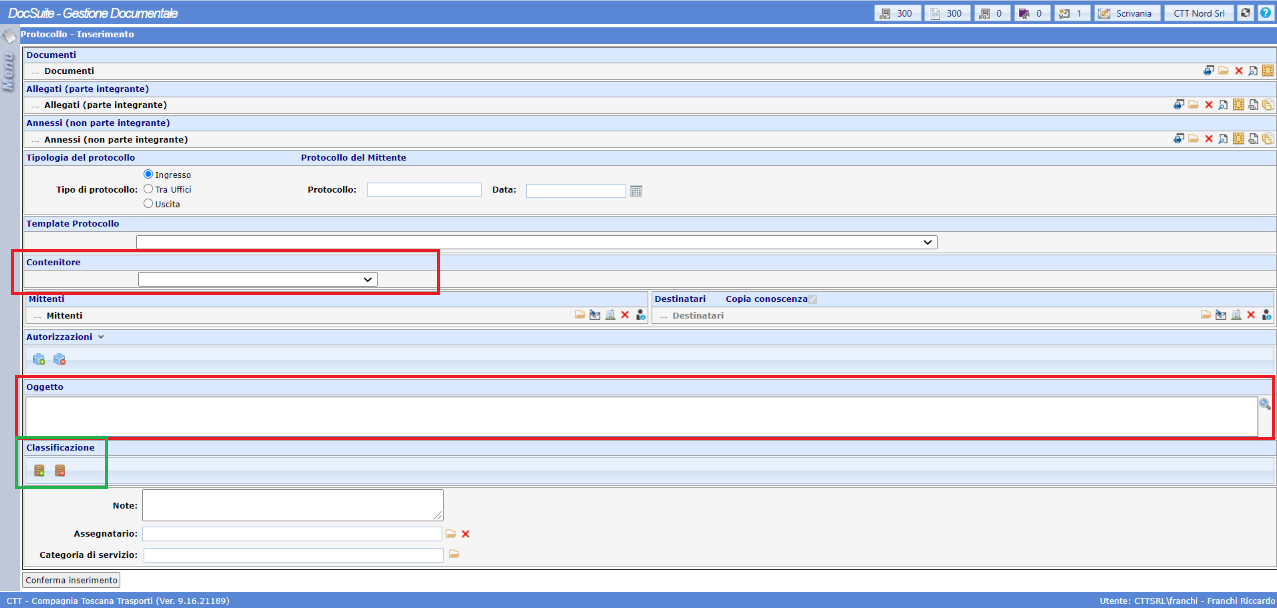
\includegraphics[width=1.5\textwidth]{interface.png}
            \end{center}
    \end{adjustwidth}
    \captionsetup{justification = centering}
    \caption{Public administration user interface}
    \label{fig:interface}
\end{figure}

\begin{figure}[ht!]
    \begin{adjustwidth}{-2cm}{}
    	    \begin{center}
        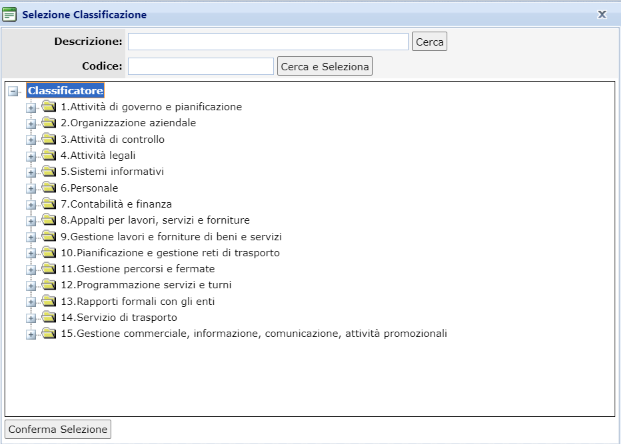
\includegraphics[width=1.3\textwidth]{class_interface.png}
            \end{center}
    \end{adjustwidth}
    \captionsetup{justification = centering}
    \caption{Classes hierarchy user interface}
    \label{fig:classinterface}
\end{figure}

\pagebreak

\begin{figure}[ht!]
        \begin{adjustwidth}{-3.2cm}{}
    	    \begin{center}
        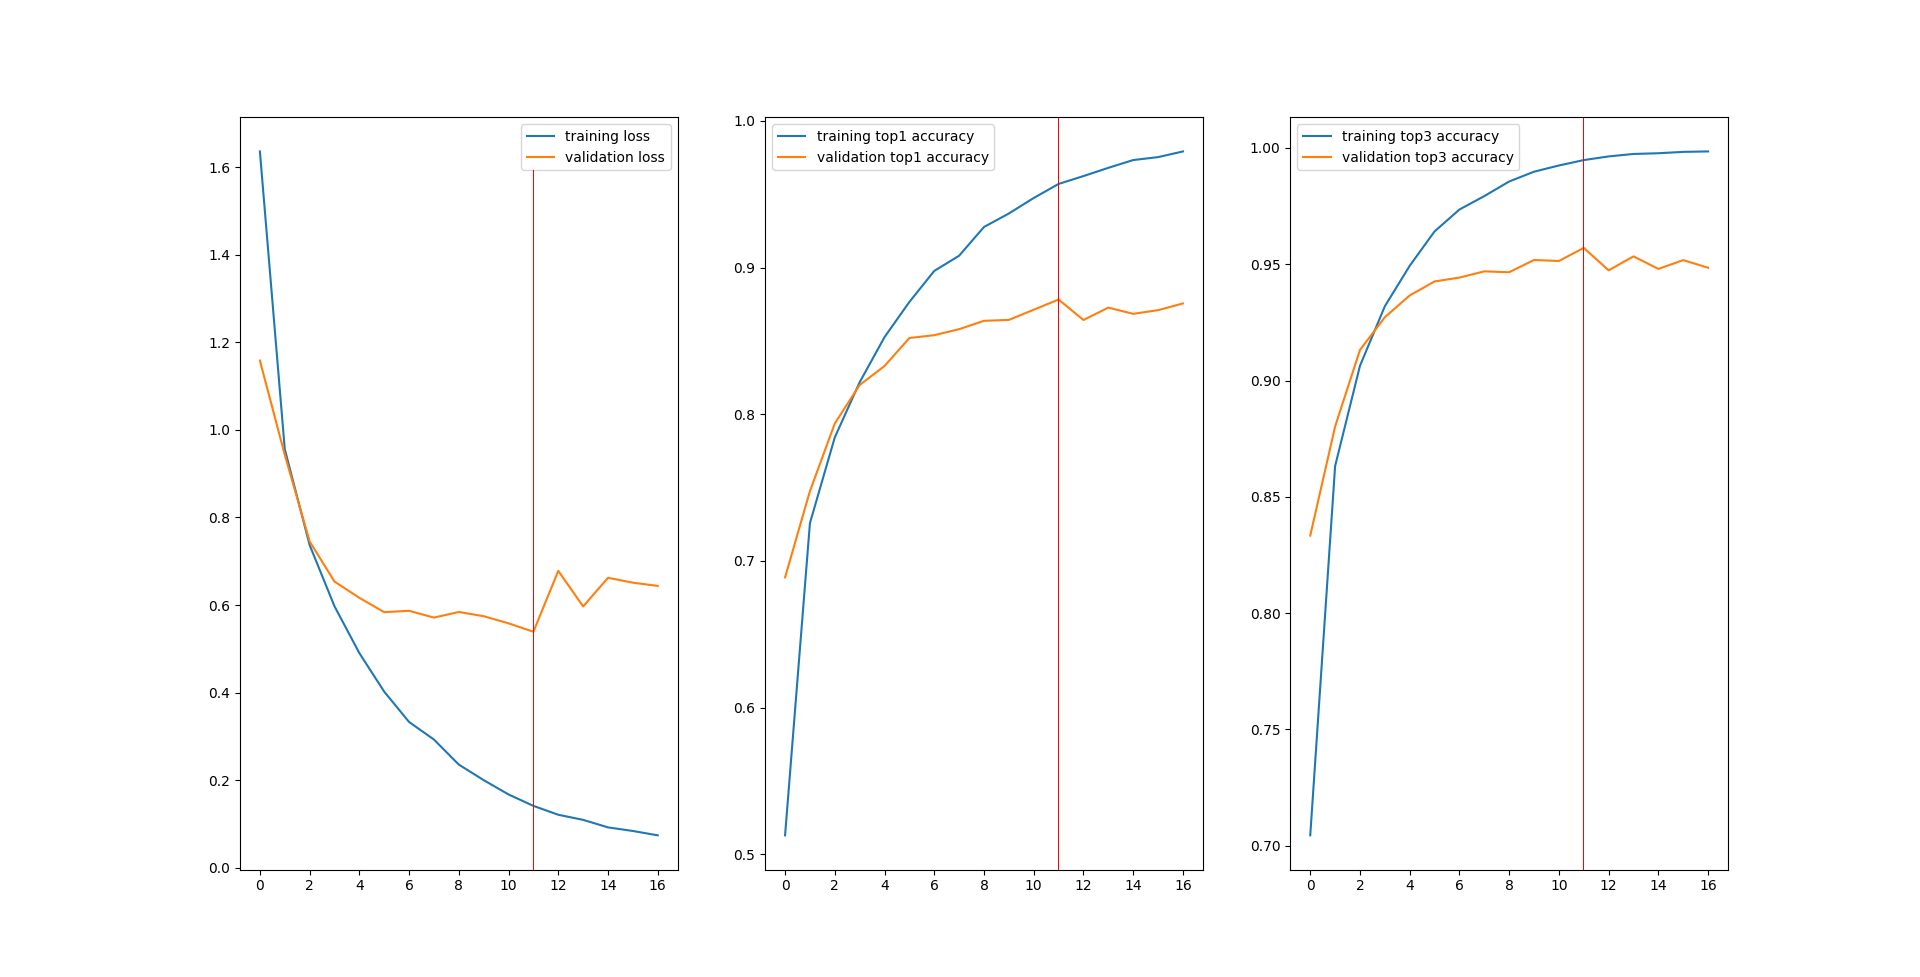
\includegraphics[width=1.5\textwidth]{#25_bar.png}
            \end{center}
	    \end{adjustwidth}
        \caption{Model 25 training/validation plots}
        \label{fig:model25}
\end{figure}

\begin{figure}[ht!]
        \begin{adjustwidth}{-3.2cm}{}
    	    \begin{center}
        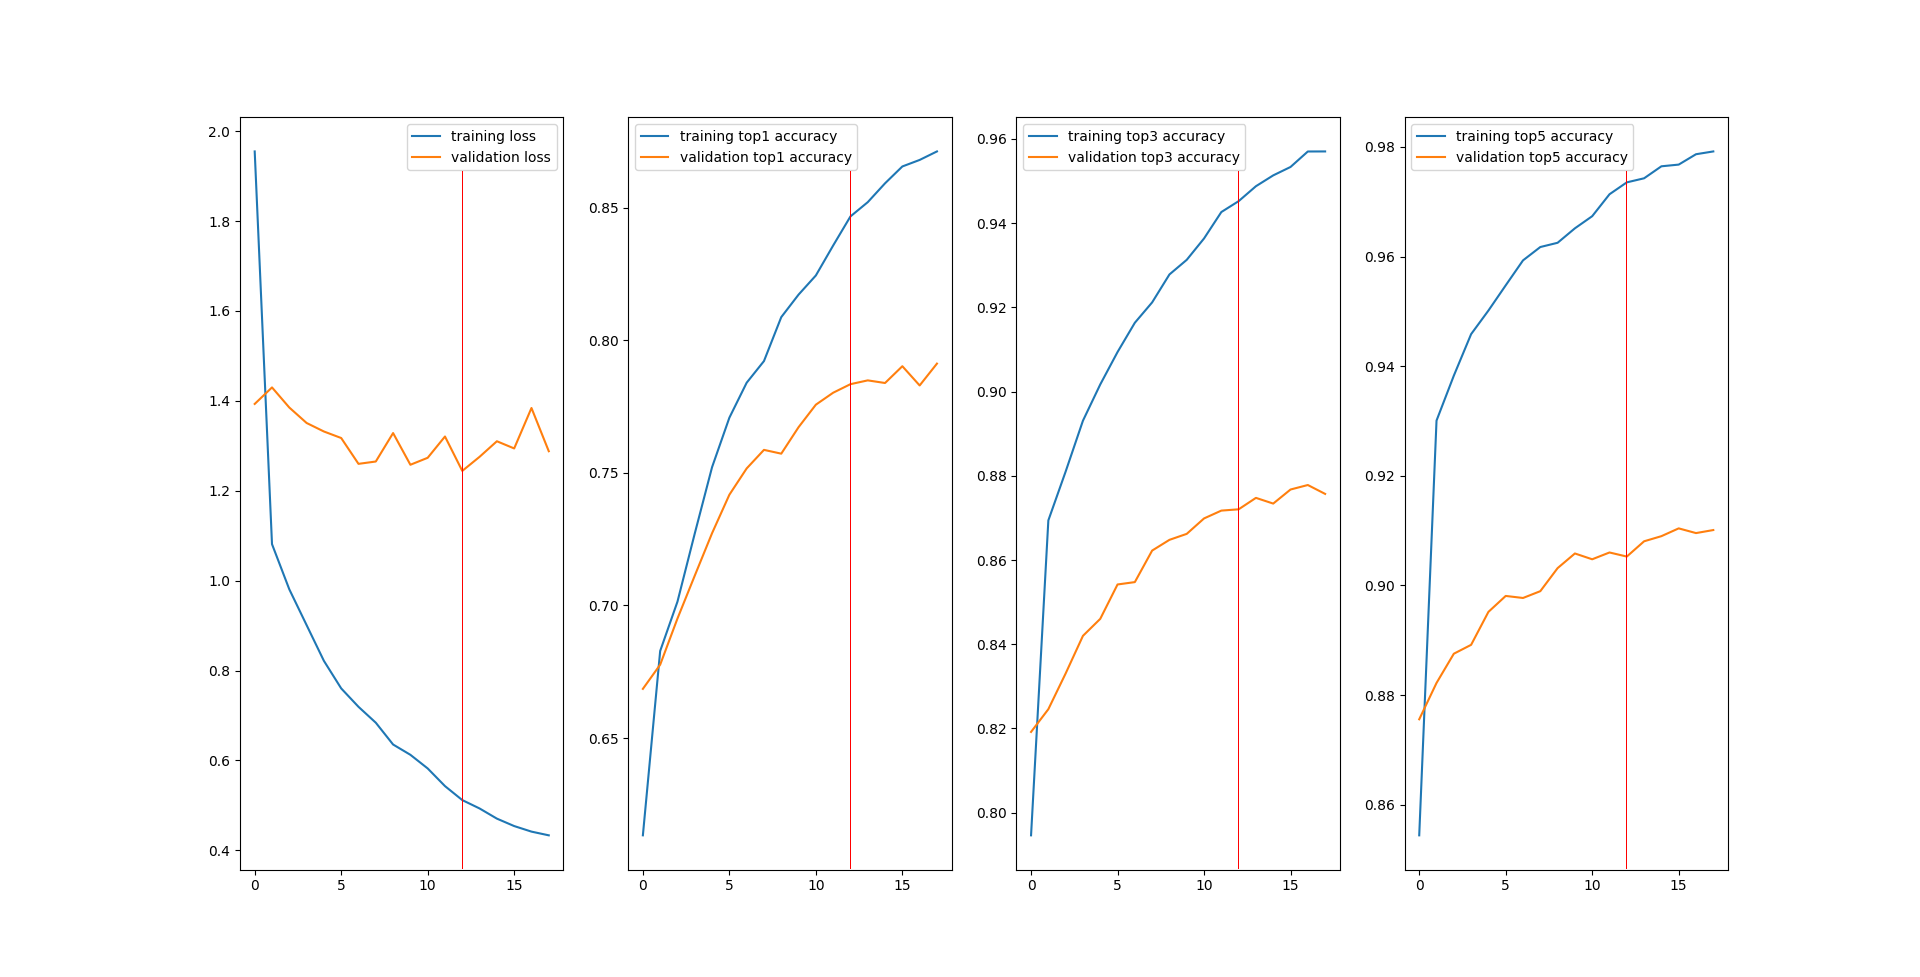
\includegraphics[width=1.5\textwidth]{#26_bar.png}
            \end{center}
	    \end{adjustwidth}
        \caption{Model 41 training/validation plots}
        \label{fig:model41}
\end{figure}
\newpage
\pagenumbering{gobble}
\begin{figure}[ht!]
        \begin{adjustwidth}{-3.2cm}{}
    	    \begin{center}
        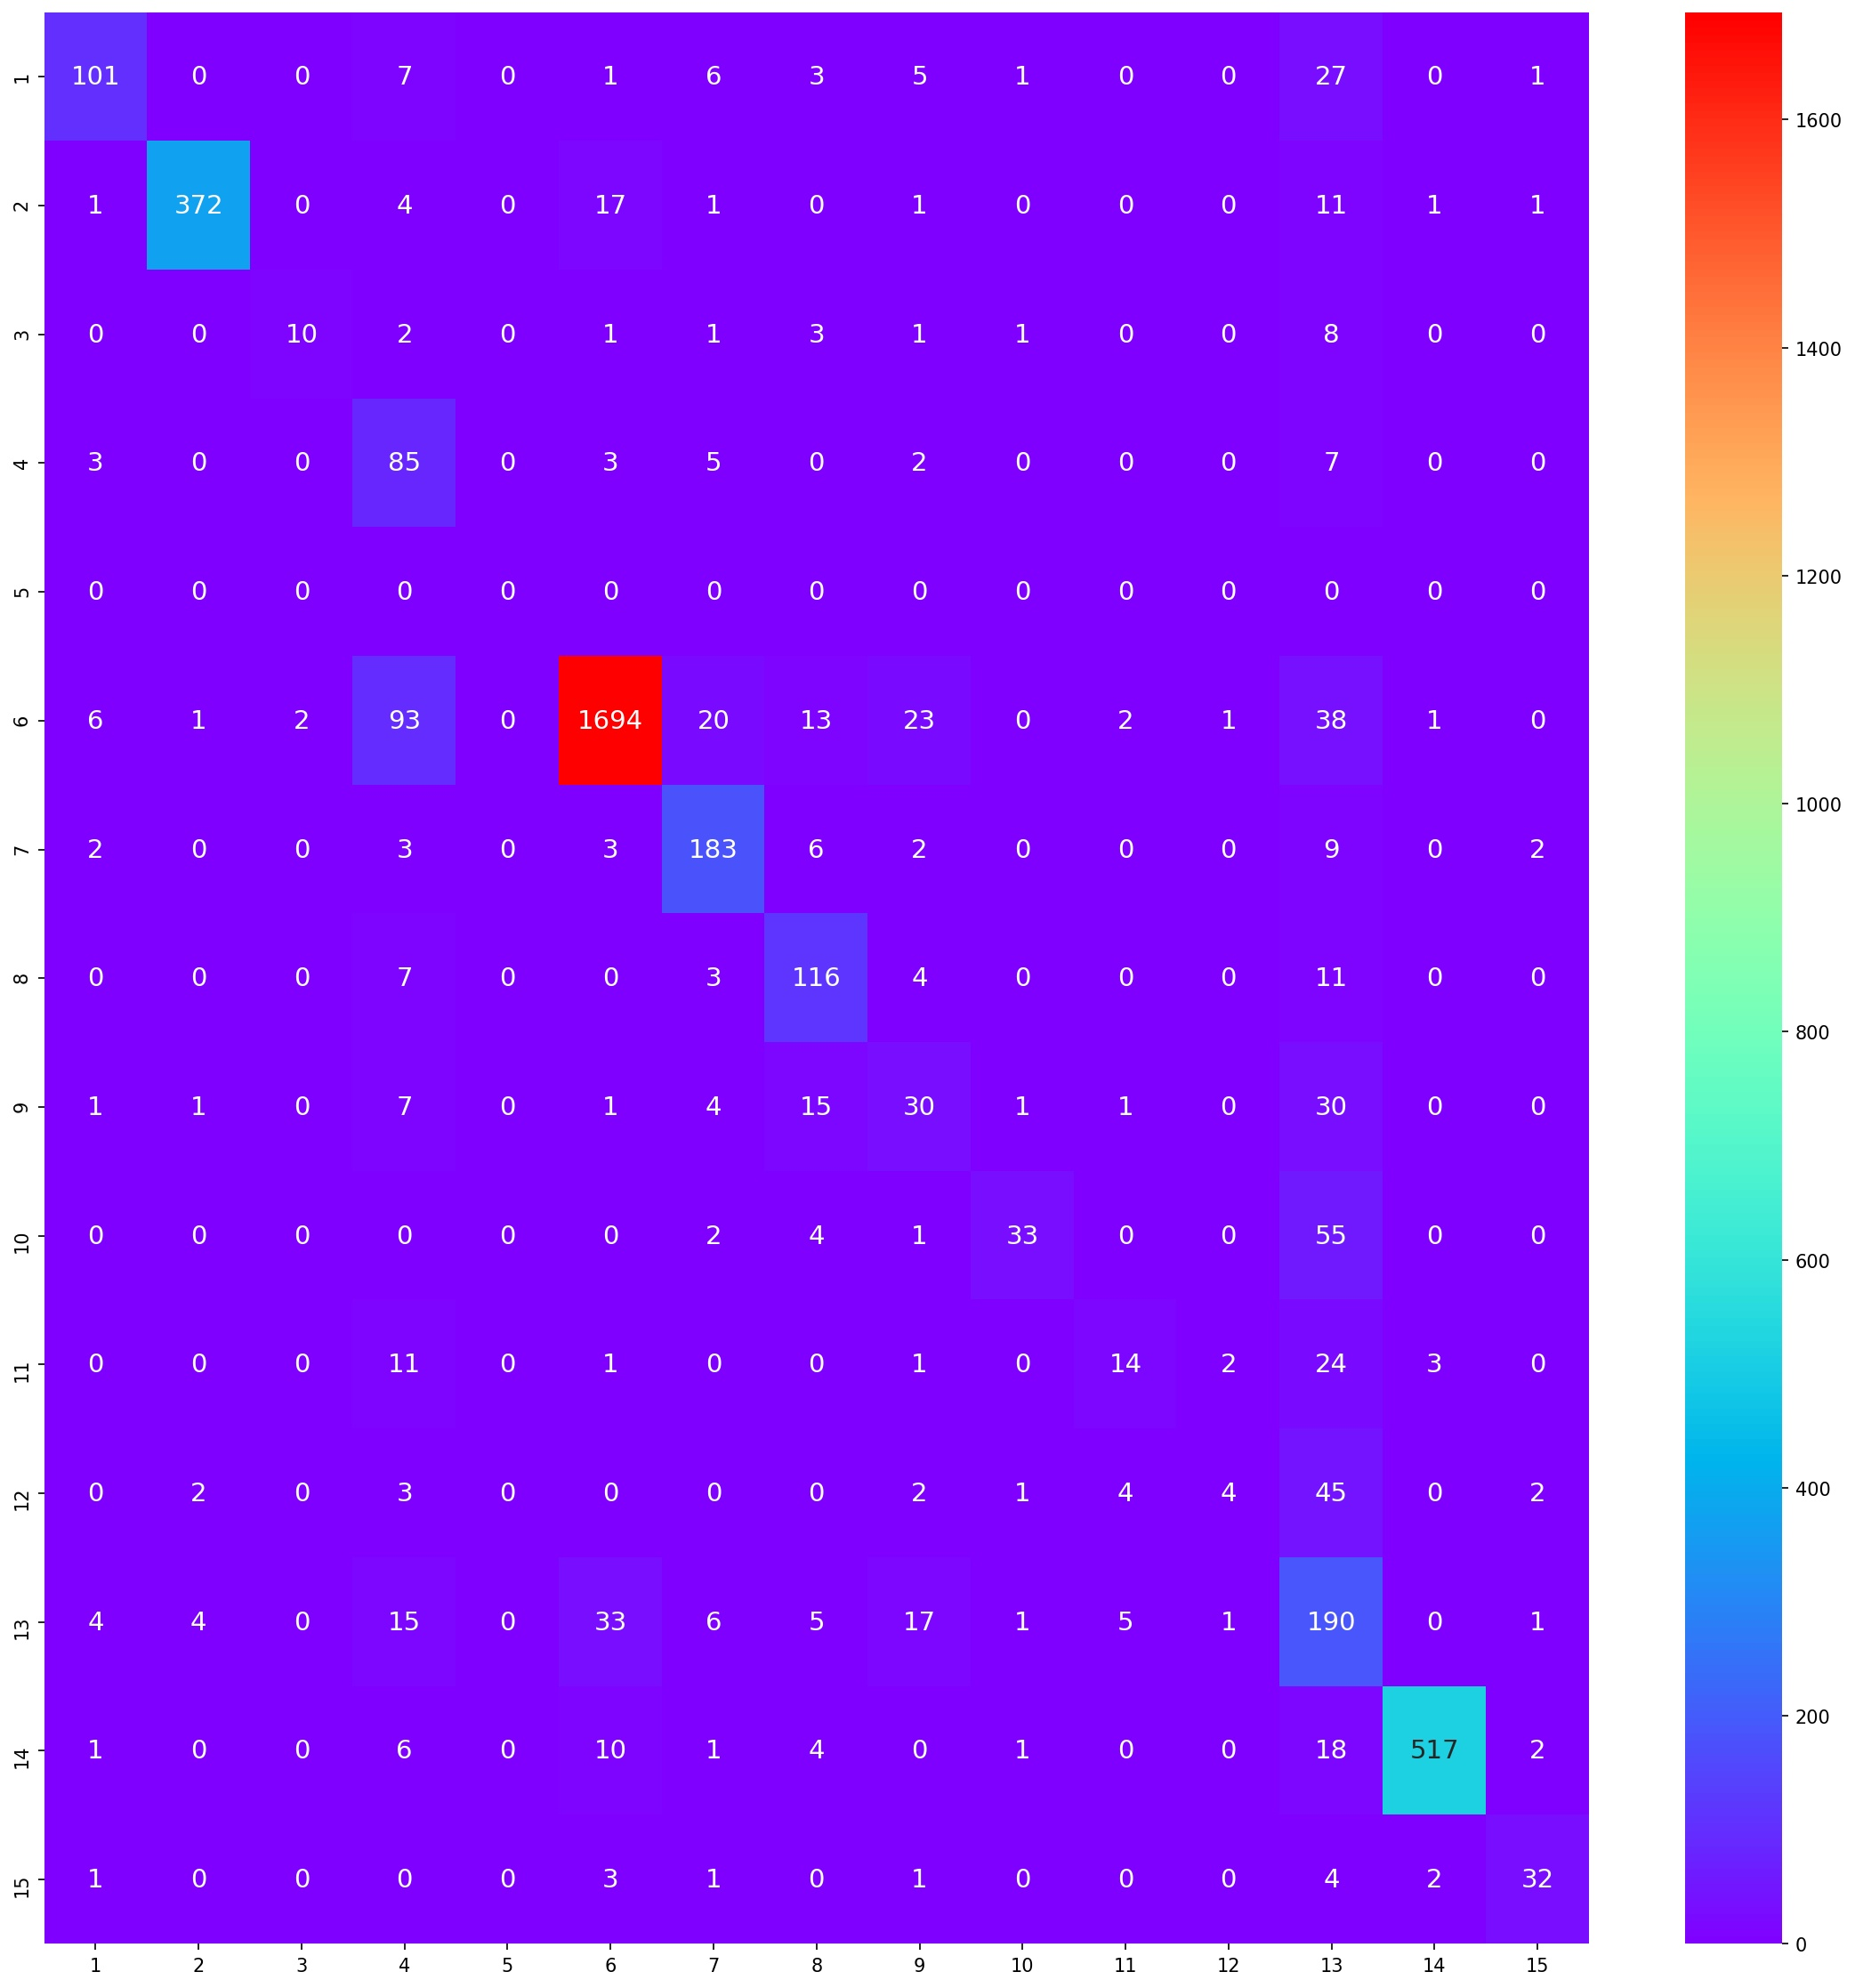
\includegraphics[width=1.45\textwidth]{heat_first.jpg}
            \end{center}
	    \end{adjustwidth}
	    \captionsetup{justification   = centering}
        \caption{Heatmap for Test Set on First level task (\textit{Top 1}) \\y axis: \textit{ground truth} - x axis: \textit{model prediction}}
        \label{fig:heatfirst1}
\end{figure}

\begin{figure}[ht!]
        \begin{adjustwidth}{-3.2cm}{}
    	    \begin{center}
        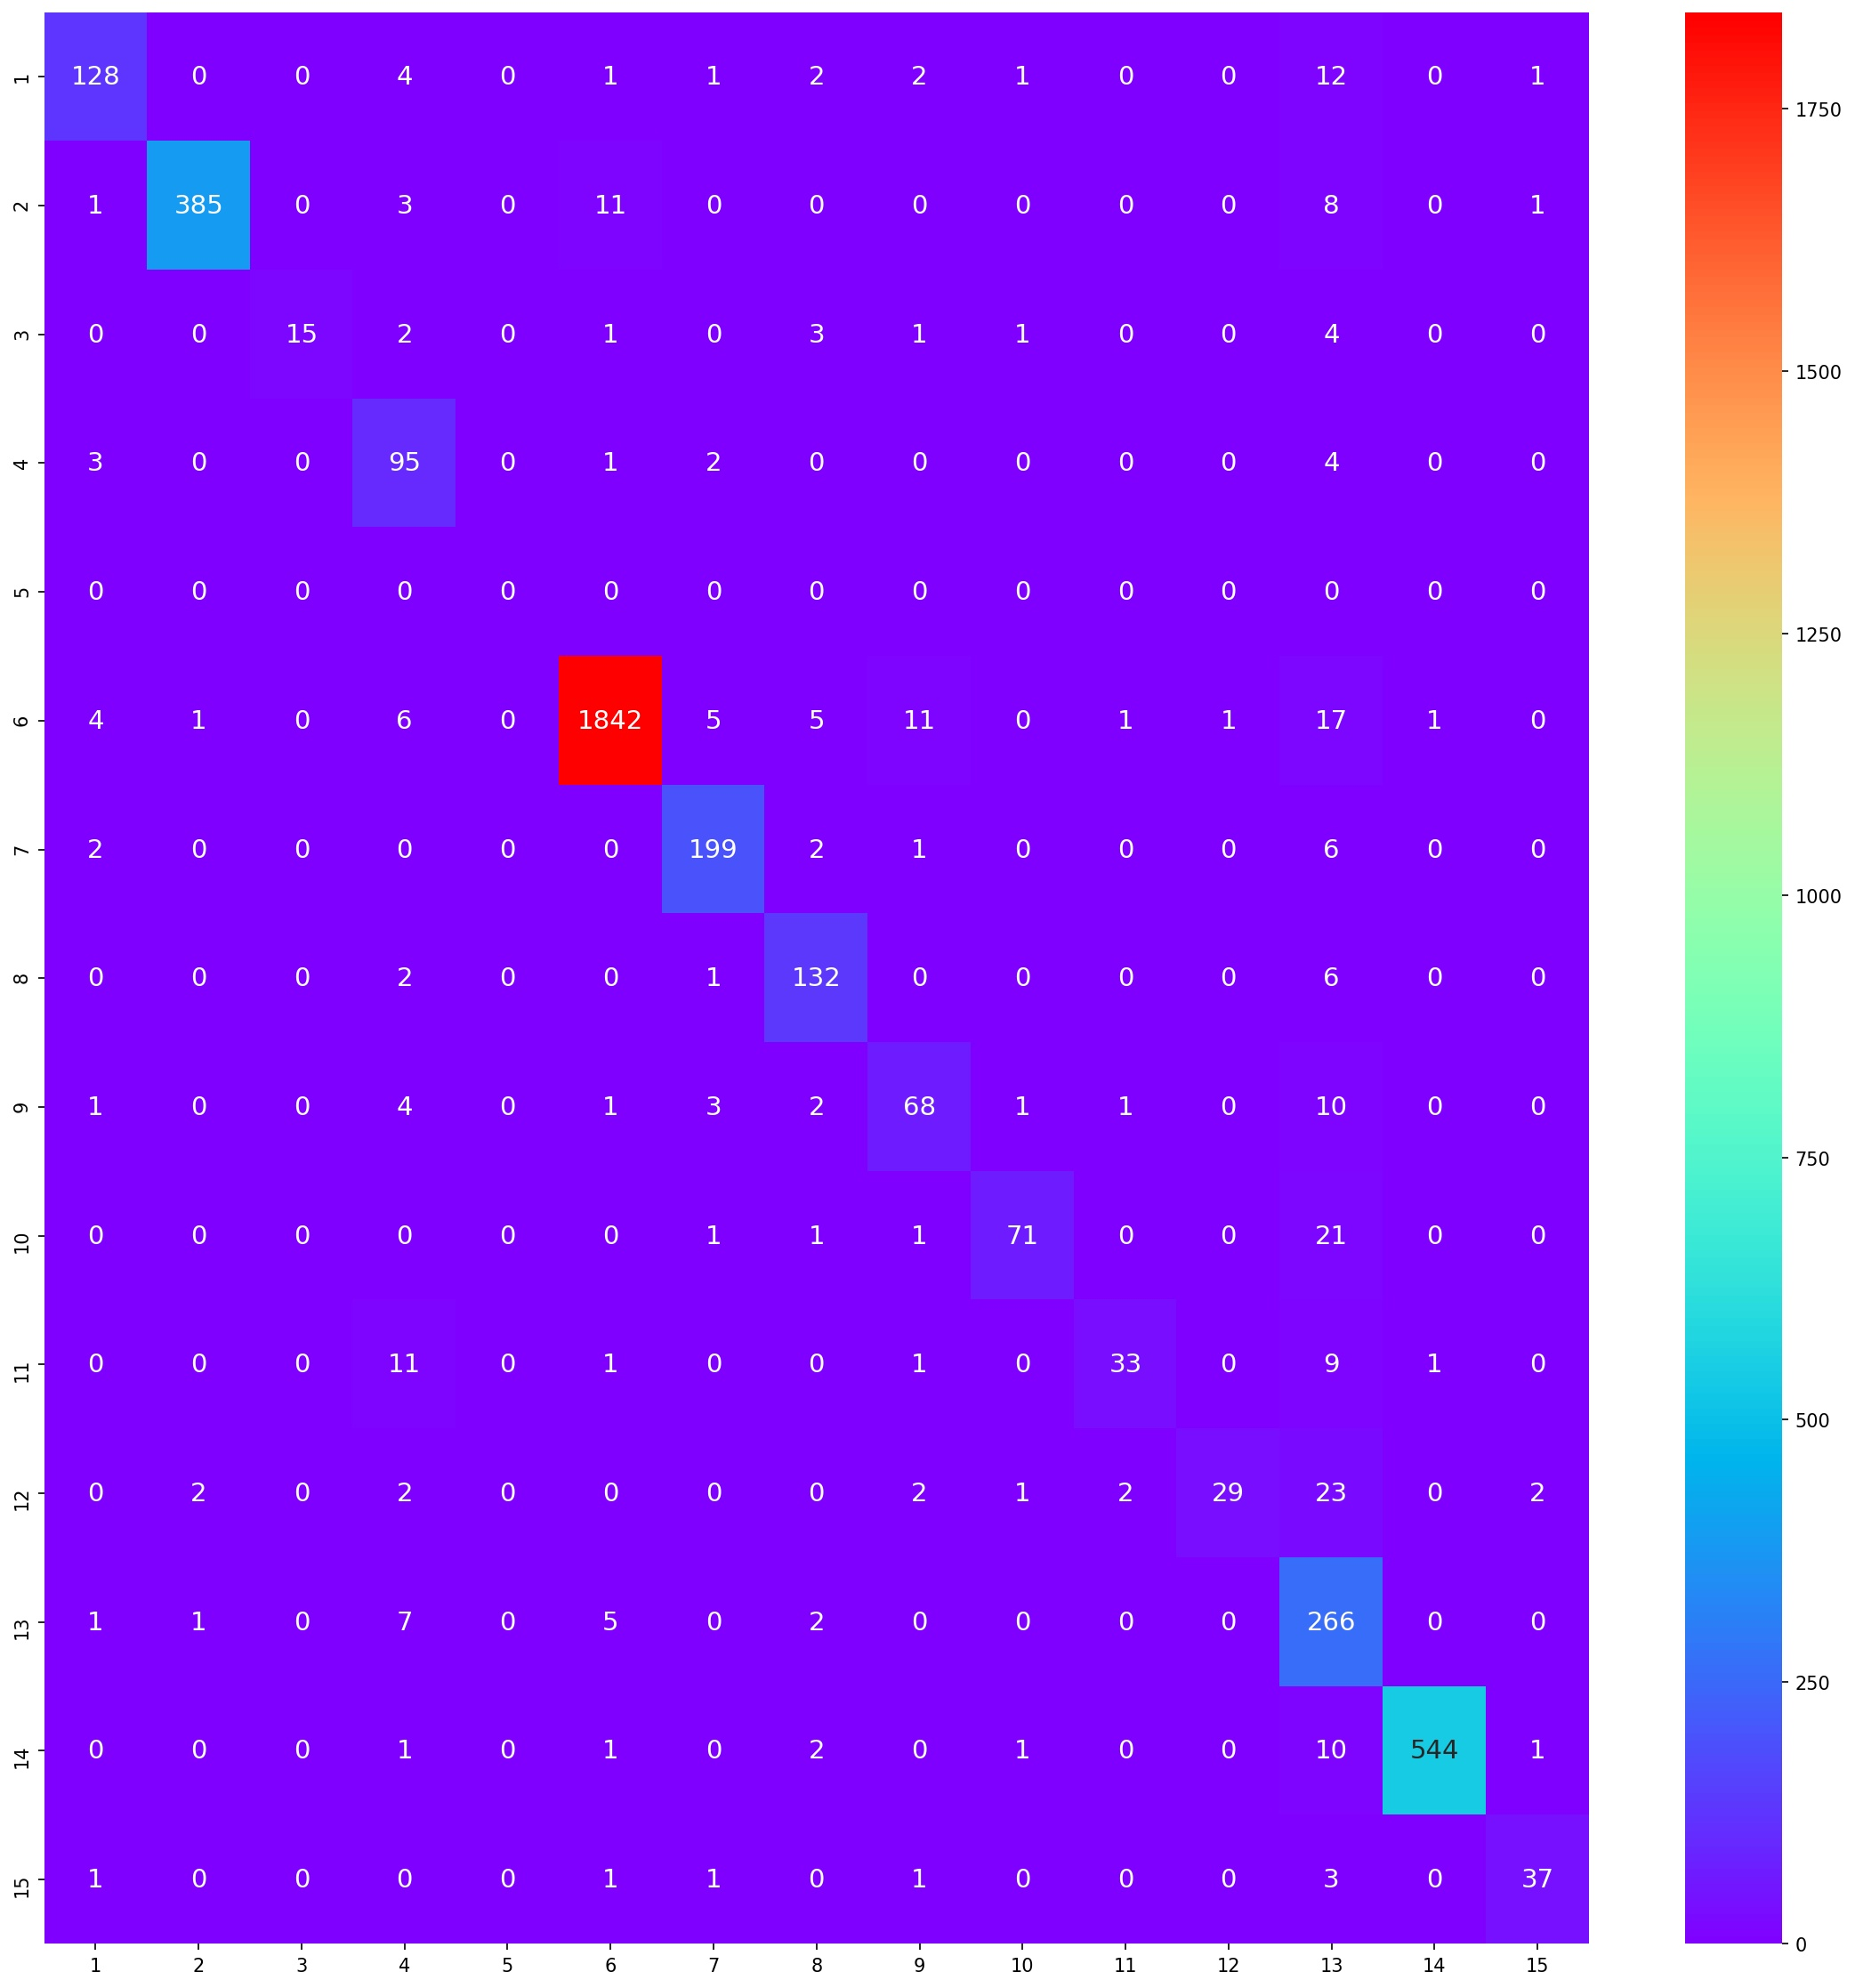
\includegraphics[width=1.45\textwidth]{heat_first3.jpg}
            \end{center}
	    \end{adjustwidth}
	    \captionsetup{justification   = centering}
        \caption{Heatmap for Test Set on First level task (\textit{Top 3) \\y axis: \textit{ground truth} - x axis: \textit{model prediction}}}
        \label{fig:heatfirst3}
\end{figure}

\begin{figure}[!tbp]
  \centering
  \subfloat[Top 1 Accuracy]{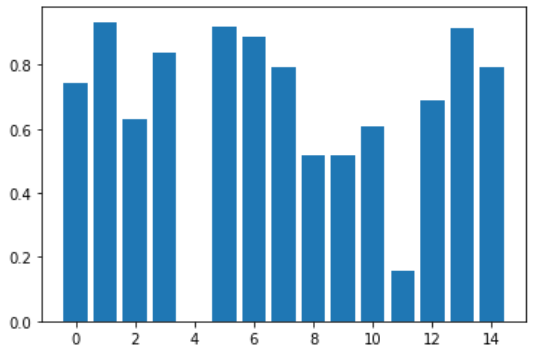
\includegraphics[width=0.4\textwidth]{class_distr1.png}\label{fig:before}}
  \hfill
  \subfloat[Top 3 Accuracy]{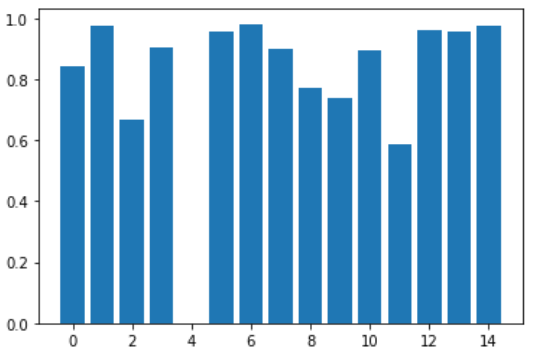
\includegraphics[width=0.4\textwidth]{class_distr3.png}\label{fig:after}}
  \captionsetup{justification   = centering}
\caption{\textit{Top 1} vs \textit{Top 3} first class task distribution \\(NB. the class are indexed starting from 0)}
\label{testclassdistrib}
\end{figure}

\begin{figure}[!tbp]
  \centering
  \subfloat[First class Top 1 accuracy ]{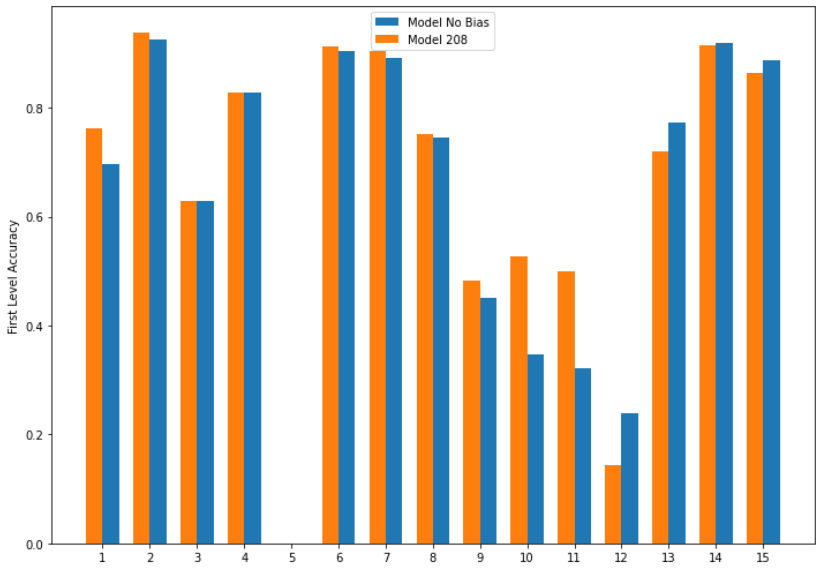
\includegraphics[width=0.6\textwidth]{acc_per_class_first_task.png}}
  \hfill
  \subfloat[Second class Top 1 accuracy ]{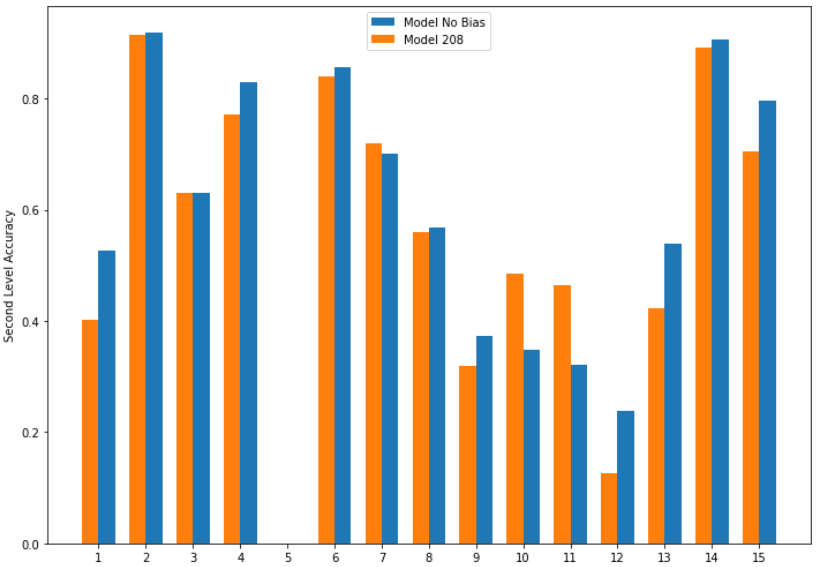
\includegraphics[width=0.6\textwidth]{acc_per_class_second_task.png}}
    \captionsetup{justification   = centering}
    \caption{\textit{First class} vs \textit{Second class} accuracy comparison between with/out bias (see \hyperref[sec:secondnobiasperformances]{\textbf{Section \ref{sec:secondnobiasperformances}}})}
\label{nobiasvs41test}
\end{figure}

\begin{figure}[!tbp]
  \centering
  \subfloat[Top 1 accuracy pieplot]{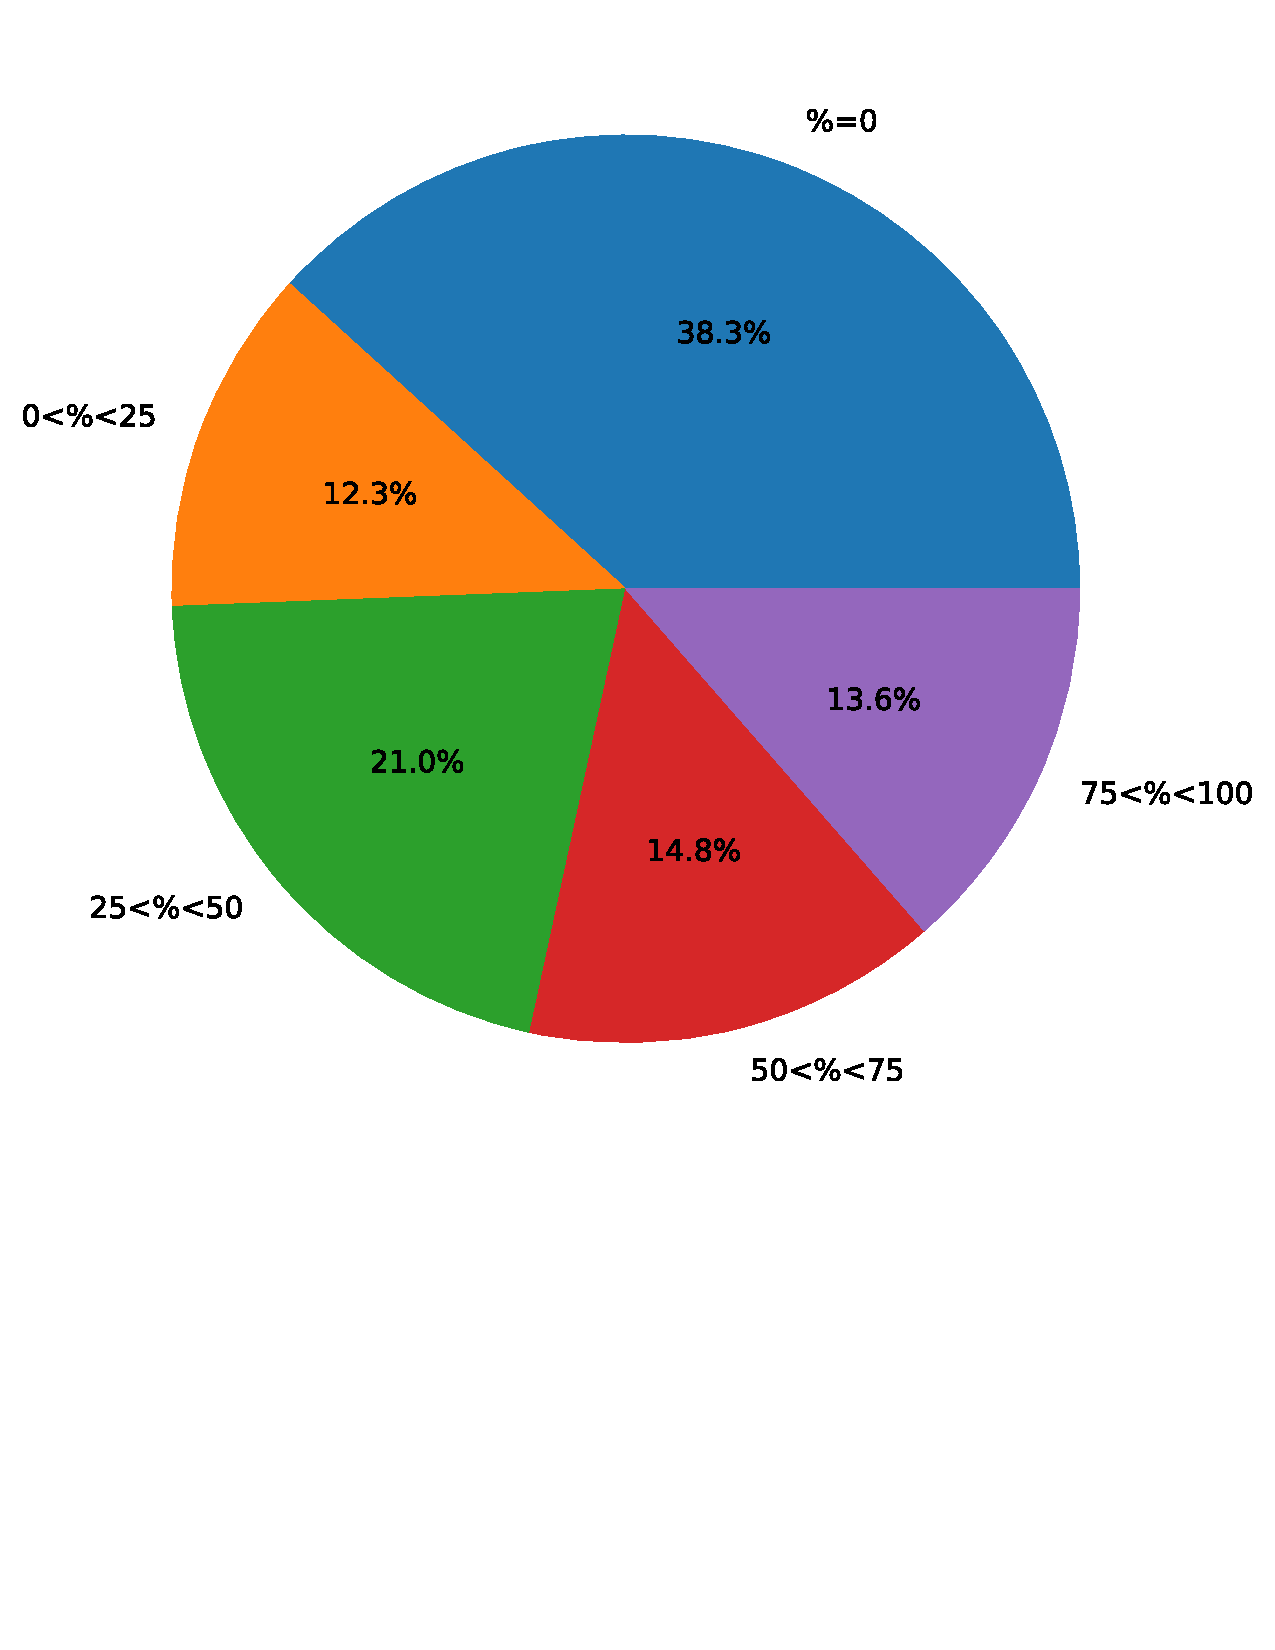
\includegraphics[width=0.55\textwidth]{pieplot1.pdf}}\label{a}
  \hfill
  \subfloat[Top 5 accuracy pieplot]{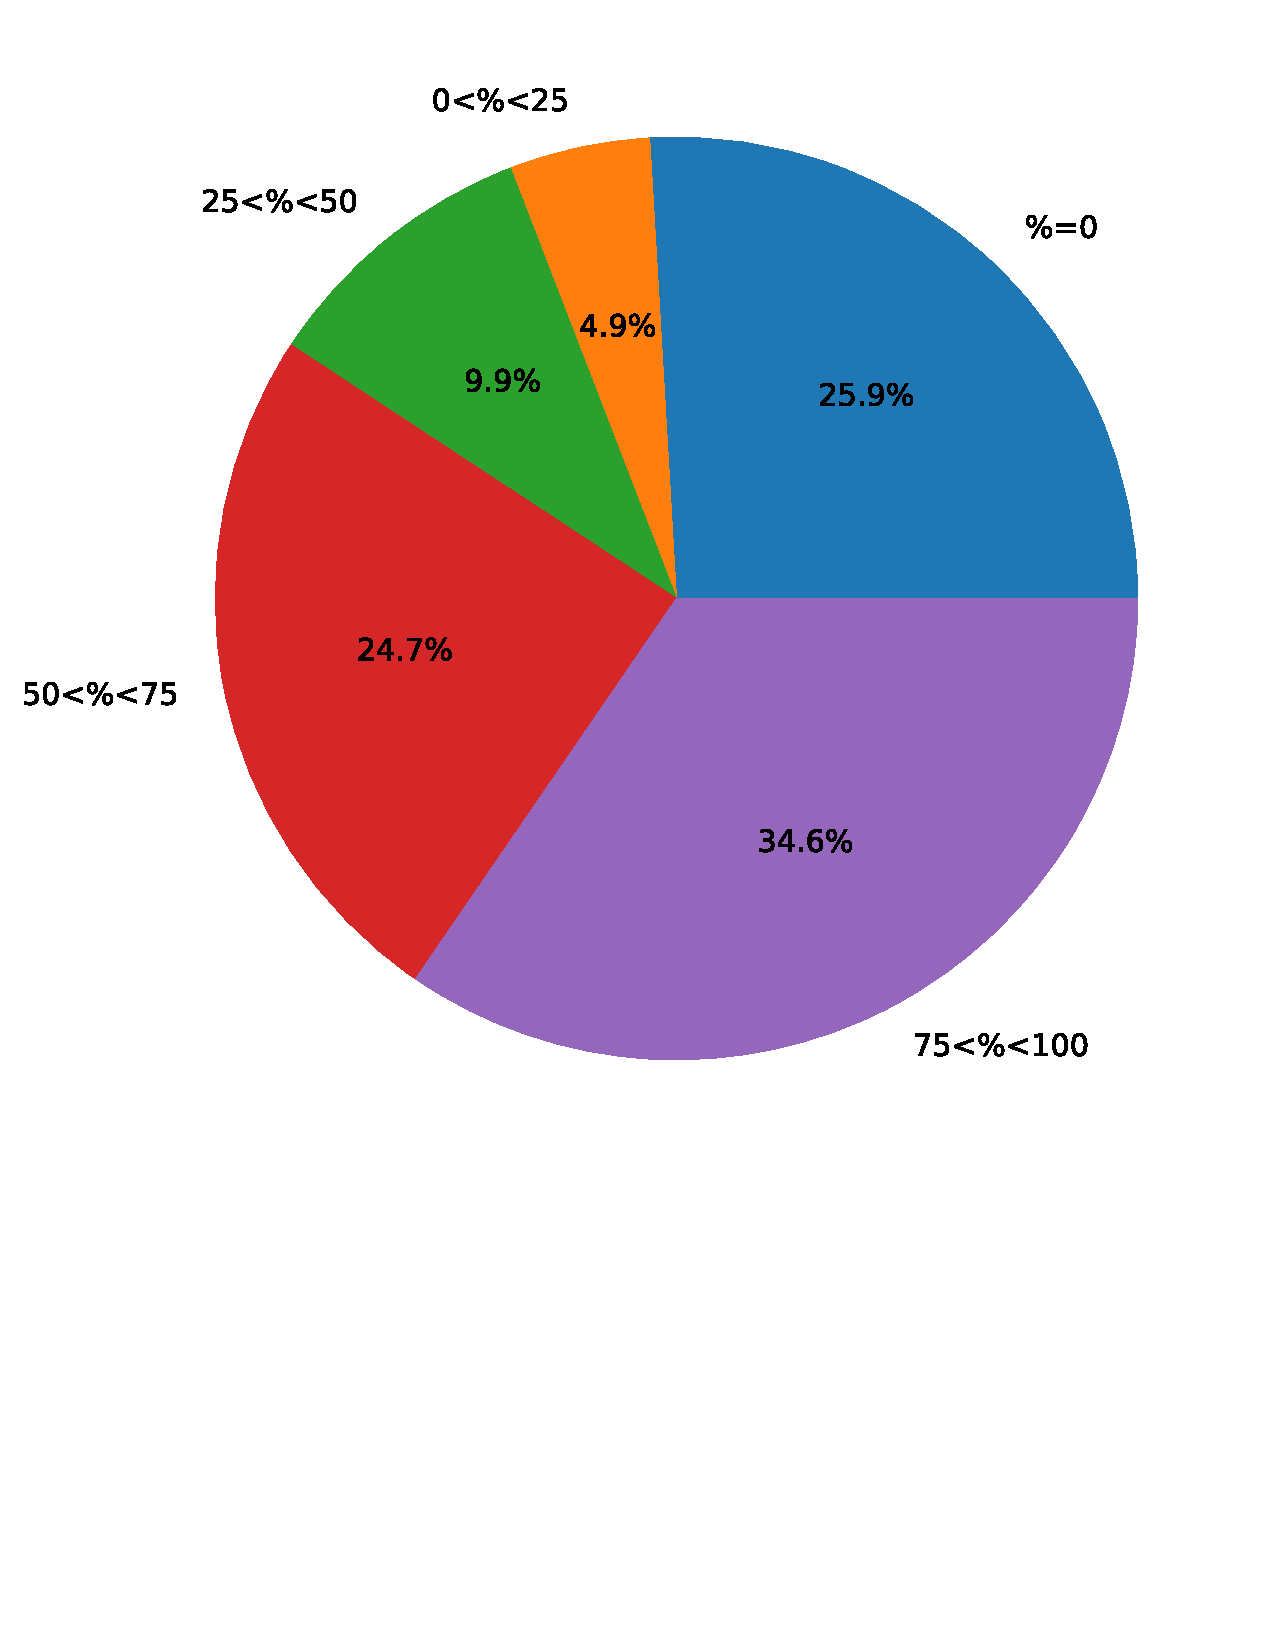
\includegraphics[width=0.55\textwidth]{pieplot5.pdf}}\label{b}
    \captionsetup{justification   = centering}
    \caption{\textit{Top 1} and \textit{Top 5} accuracy pieplots for Second Level Task testing}
\label{pieplot}
\end{figure}
\end{document}